\section{Model epidemije}

Za simulacijo okužbe neke populacije lahko uporabimo preprost model na osnovi sistema dveh navadnih diferencialnih enačb, kjer so $D$ zdravi, a za okužbo dovzetni osebki in $B$ bolni/okuženi
\begin{align}\label{eqn:1}
    \dot D &= -\alpha \, D \, B \\ \nonumber
    \dot B &= \alpha \, D \, B
\end{align}
Takšen preprost model omogoča le modeliranje širjenja okužbe, ne upošteva pa ozdravitve ali smrti obolelega. Tako bi bilo primerno modelirati nesmrtne kronične okužbe, ki se jih tudi ne zdravi, kot je npr. širjenje virusa \textit{herpes} ali \textit{HPV} po populaciji.

Model lahko nadgradimo z uvedbo nove -- imune skupine $I$, tokrat rešujemo sistem treh navadnih DE
\begin{align}\label{eqn:2}
    \dot D &= -\alpha \, D \, B & \dot D &= -R_0 \, D \, B \\ \nonumber
    \dot B &= \alpha \, D \, B - \beta \, B  & \dot B &= R_0 \, D \, B - B\\ \nonumber
    \dot I &= \beta \, B  & \dot I &= B
\end{align}
Z uvedbo reprodukcijskega števila $R_0 = \alpha / \beta$ kot razmerja med ‘hitrostjo’ okuževanja in ozdravljenja, ki opisuje hitrost širjenja bolezni lahko rešujemo sistem le z eno konstanto. To število tudi določa končno ustaljeno stanje bolezni. Na tak način se lahko modelira prekuženost populacije pri npr. ošpicah, kjer so preboleli osebki tudi imuni do konca življenja.

Lahko spremenimo model tako, da preboleli osebki ne postanejo imuni, temveč so ponovno zdravi, vendar dovzetni za okužbo
\begin{align}\label{eqn:3}
    \dot D &= -\alpha \, D \, B + \beta \, B & \dot D &= -R_0 \, D \, B + B \\ \nonumber
    \dot B &= \alpha \, D \, B - \beta \, B & \dot B &= R_0 \, D \, B - B
\end{align}
Spremenjeni model omogoča modeliranje  bolezni, ki so stalno prisotne v populaciji, vendar niso smrtne, kot je npr. virus prehlada ali nekatere spolno prenosljive bolezni, kot je npr. gonoreja.

Če uvedemo novo konstanto $\gamma$, lahko z njo opišemo prehajanje imunih oseb nazaj v populacijo dovzetnih, vendar tokrat z uvedbo razmerja imunosti $I_0 = \gamma / \beta$, ki opisuje hitrost prehajanja imunih nazaj v dovzetne, ne uspemo zmanjšati števila konstant.
\begin{align}\label{eqn:4}
    \dot D &= -\alpha \, D \, B & \dot D &= -R_0 \, D \, B + I_0 \, I\\ \nonumber
    \dot B &= \alpha \, D \, B - \beta \, B & \dot B &= R_0 \, D \, B -B \\ \nonumber
    \dot I &= \beta \, B - \gamma \, I & \dot I &= B - I_0 \, I 
\end{align}
Tako lahko še bolj realno popišemo epidemijo, kjer obstaja imuno stanje, ki pa ne traja večno.

V želji po opisu tudi smrtnih okužb uvedemo novo skupino umrlih $M$ in koeficient umrljivosti $\delta$, ki velja le za obolele osebke. Pri normiranju tako dobimo razmerje umrljivosti $M_0 = \delta / \beta$. S tem smo zagotovili pogoje matematično konstantne populacije.
\begin{align}\label{eqn:5}
    \dot D &= -\alpha \, D \, B & \dot D &= -R_0 \, D \, B + I_0 \, I\\ \nonumber
    \dot B &= \alpha \, D \, B - \beta \, B - \delta \, B & \dot B &= R_0 \, D \, B - B - M_0 \, B \\ \nonumber
    \dot I &= \beta \, B - \gamma \, I & \dot I &= B - I_0 \, I \\ \nonumber
    \dot M &= \delta B & \dot M &= M_0 \, B
\end{align}

Ob upoštevanju rojstev lahko naredimo populacijo nekostantne velikosti. To zadovoljimo z uvedbo konstante $\varepsilon$, ki ob normiranju postane razmerje rojstev $N_0 = \varepsilon / \beta$. Le-to velja za populaciji imunih in dovzetnih, ob predpostavkama, da se bolni ne ‘množijo’ in da so novi osebki dovzetni na okužbo.
\begin{align}\label{eqn:6}
    \dot D &= -\alpha \, D \, B + \varepsilon \, (D+I) & \dot D &= -R_0 \, D \, B + I_0 \, I + N_0 \, (D+I)\\ \nonumber
    \dot B &= \alpha \, D \, B - \beta \, B - \delta \, B & \dot B &= R_0 \, D \, B - B - M_0 \, B \\ \nonumber
    \dot I &= \beta \, B - \gamma \, I & \dot I &= B - I_0 \, I \\ \nonumber
    \dot M &= \delta B & \dot M &= M_0 \, B
\end{align}

Dodatno lahko uvedemo več stadijev epidemije, zapisan je primer za 3 stadije, kjer z različnimi koeficienti $\beta$ uravnavamo kužnost bolezni.
\begin{align}\label{eqn:6}
    \dot D &= -\alpha \, D \, B_1 + \varepsilon \, (D+I) \\ \nonumber
    \dot B_1 &= \alpha \, D \, B_1 - \beta_1 \, B_1 - \delta \, B_1 \\ \nonumber
    \dot B_2 &=  \beta_1 \, B_1- \beta_2 \, B_2 - \delta \, B_2 \\ \nonumber
    \dot B_3 &=  \beta_2 \, B_2 - \beta_3 \, B_3 - \delta \, B_3 \\ \nonumber
    \dot I &= \beta \, B - \gamma \, I \\ \nonumber
    \dot M &= \delta B
\end{align}
Na tak način smo dobili že sistem 6 navadnih DE, ki pa vseeno ni težko rešljiv. Reševali smo ga v \texttt{Python}-u s pomočjo funkcije \texttt{scipy.integrate.odeint}, ki rešuje sistem NDE z algoritmom lsoda iz \texttt{FORTRAN}-ove knjižnice.

\begin{figure}[ht!]
\begin{centering}
    \begin{subfigure}[b]{0.5\textwidth}\label{fig:okužba}
        \centering
        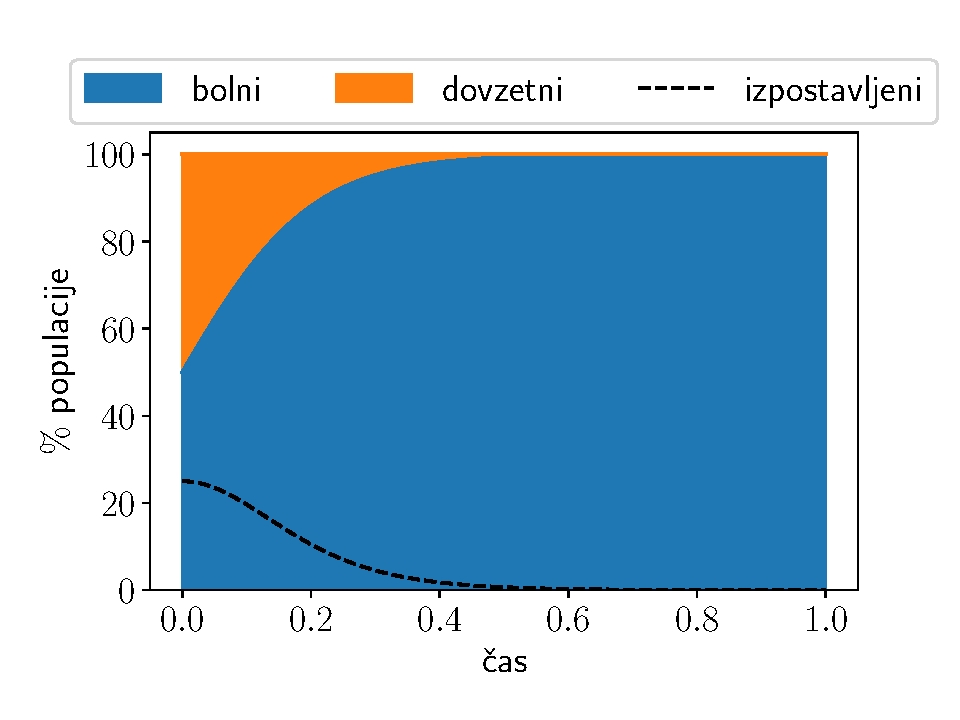
\includegraphics[width=\linewidth]{4.nal slike/okužba.pdf}
        \caption{Po enačbi \ref{eqn:1} za $\alpha = 1$, 930 obolelih}
    \end{subfigure}
    \begin{subfigure}[b]{0.5\textwidth}\label{fig:imunost}
        \centering
        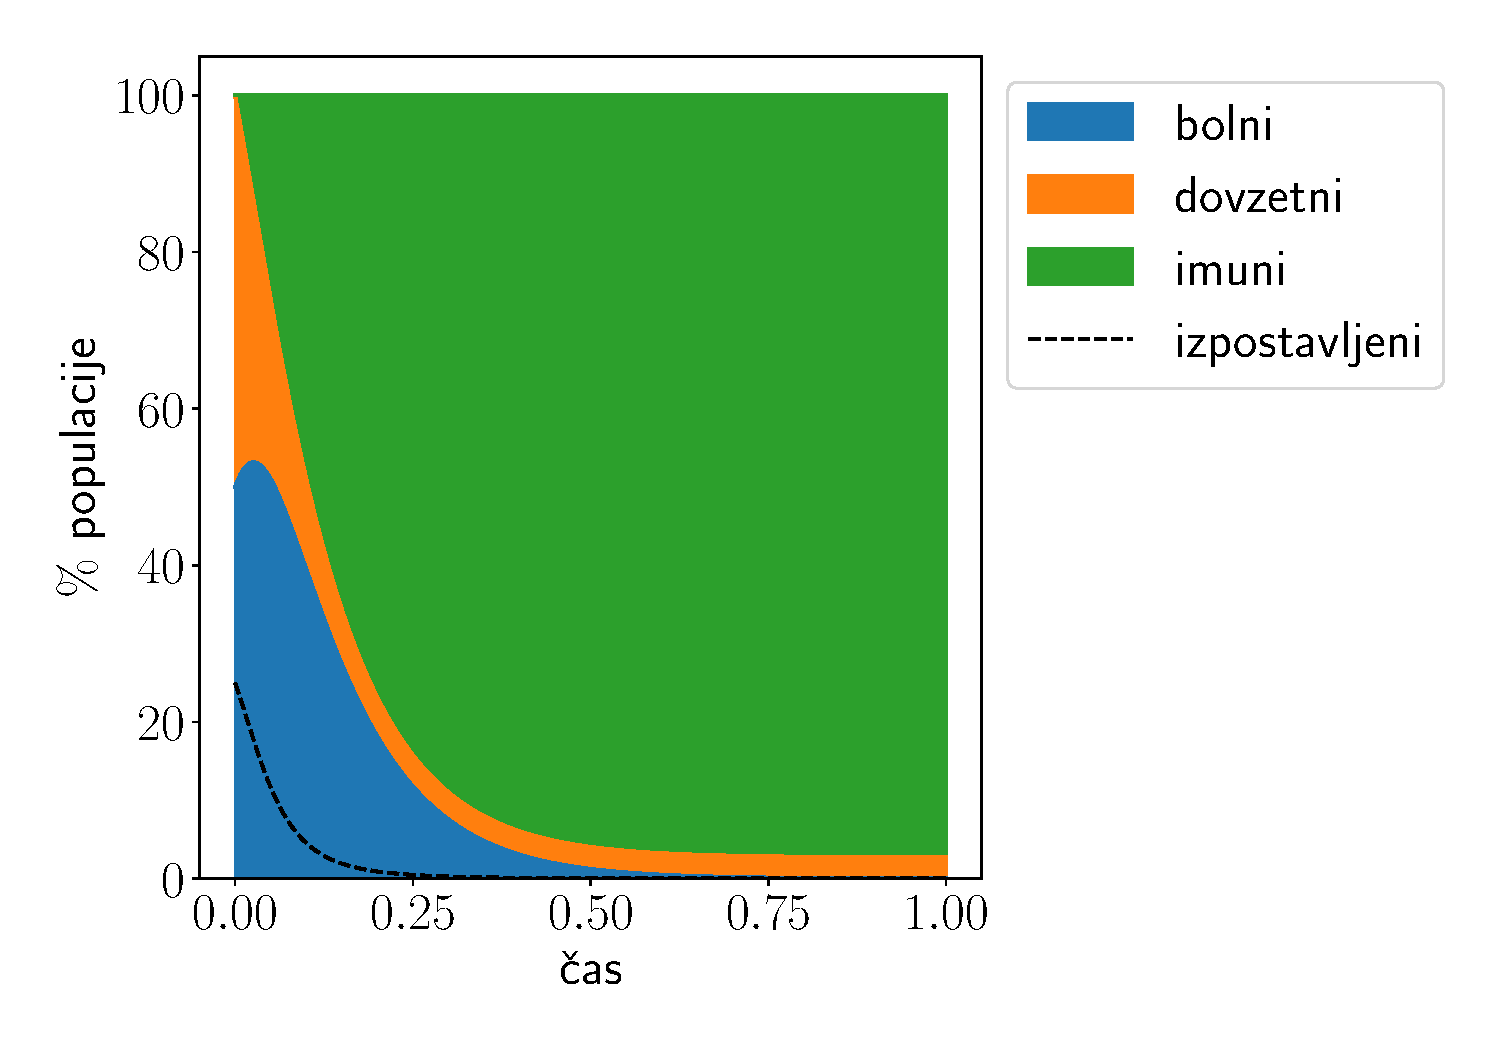
\includegraphics[width=\linewidth]{4.nal slike/imunost.pdf}
        \caption{Po enačbi \ref{eqn:2} za $R_0 = 3$, 97 obolelih, vrh pri 53,2 \% in $\tau=0,026$}
    \end{subfigure}
    \begin{subfigure}[b]{0.5\textwidth}
        \centering
        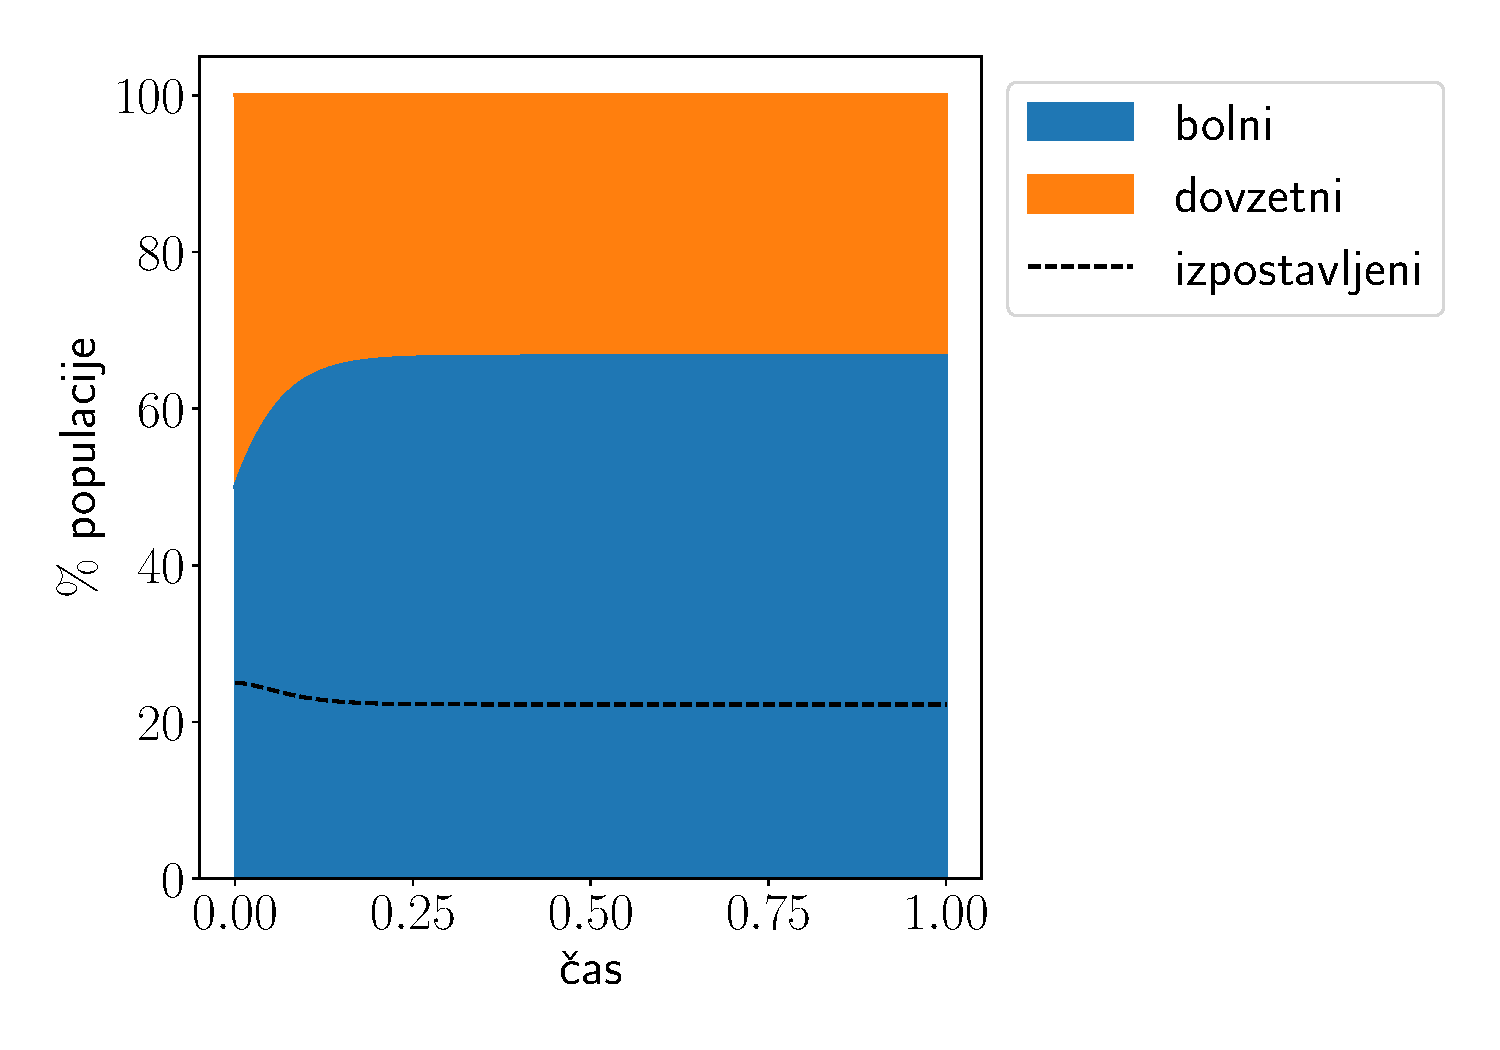
\includegraphics[width=\linewidth]{4.nal slike/ne-imunost.pdf}
        \caption{Po enačbi \ref{eqn:3} za $R_0 = 3$, 657 obolelih, stabilizacija pri 66,7 \%}
        \label{fig:ne-imunost}
    \end{subfigure}
    \begin{subfigure}[b]{0.5\textwidth}
        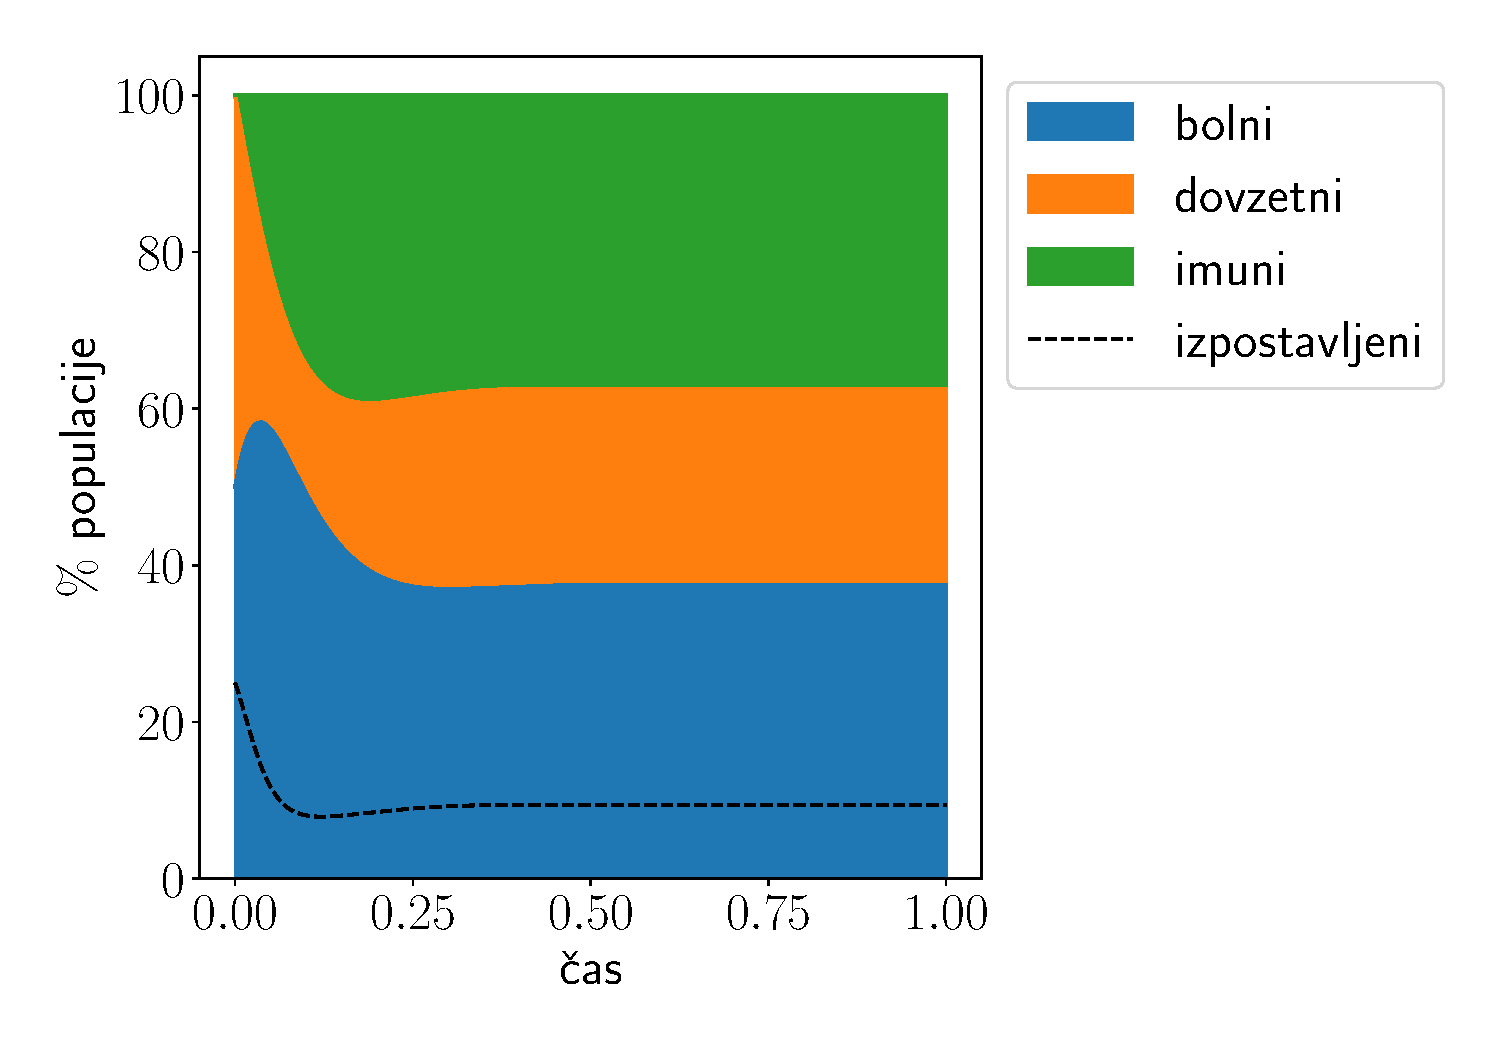
\includegraphics[width=\linewidth]{4.nal slike/ozdravitev.pdf}
        \caption{Po enačbi \ref{eqn:4} za $R_0 = 4$ in $I_0 = 1$, obolelih 397, vrh 58,3 \% in $\tau=0,36$}
        \label{fig:ozdravitev}
    \end{subfigure}
\end{centering}
\caption{Simulacije epidemije po različnih modelih}
\end{figure}
\begin{figure}[ht!]
\begin{centering}
    \begin{subfigure}[b]{0.5\textwidth}
        \centering
        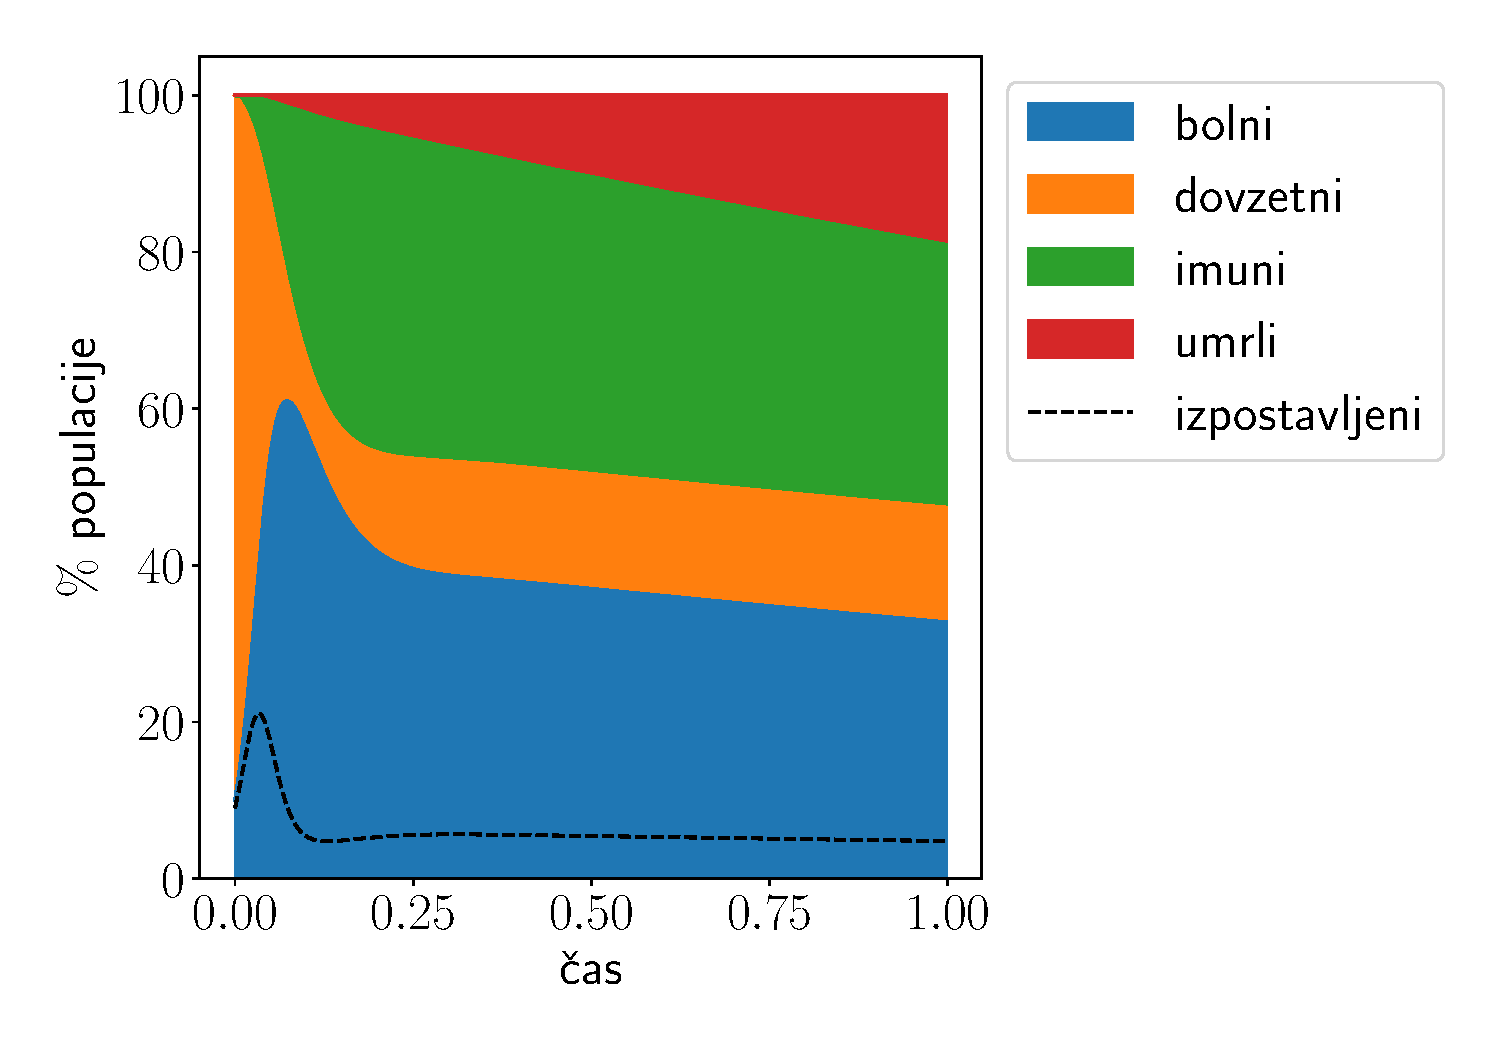
\includegraphics[width=\linewidth]{4.nal slike/smrti.pdf}
        \caption{Simulacija po enačbi \ref{eqn:5} za $R_0 = 7$,$I_0=1$,$M_0=0,05$}
        \label{fig:smrti}
    \end{subfigure}
    \begin{subfigure}[b]{0.5\textwidth}
        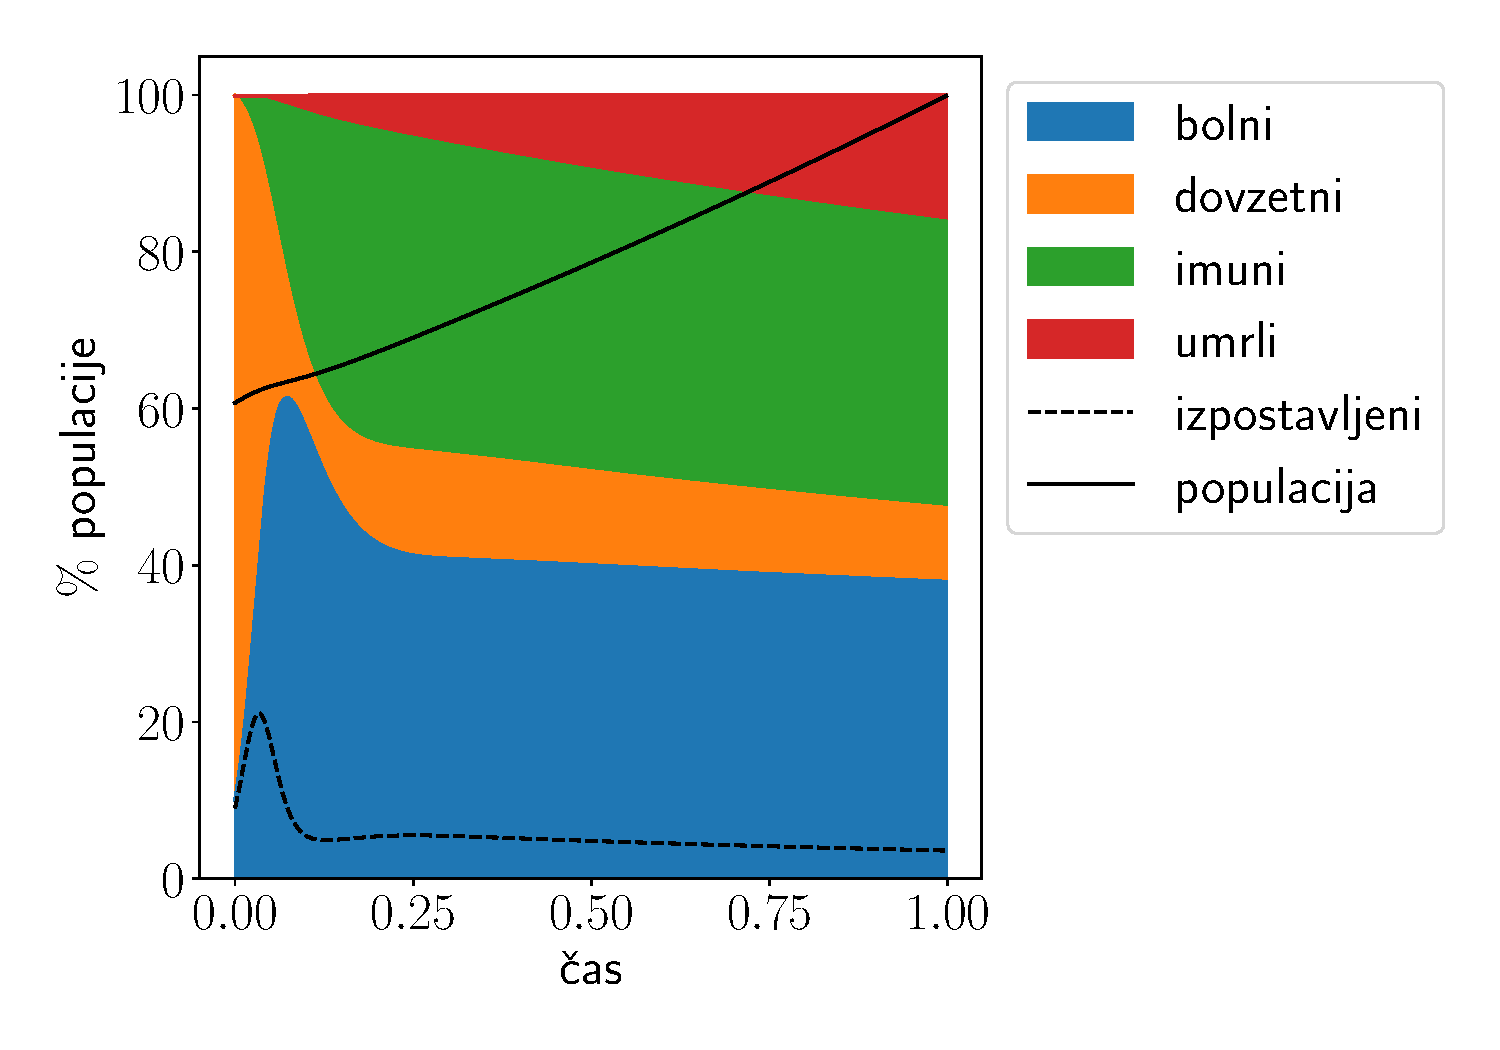
\includegraphics[width=\linewidth]{4.nal slike/smrti_rojstva.pdf}
        \caption{Simulacija po enačbi \ref{eqn:6} upoštevajoč tudi rojstva za $R_0 = 7$,$I_0=1$,$M_0=0,05$ in $N_0=0,1$}
        \label{fig:smrti_rojstva}
    \end{subfigure}
\end{centering}
\caption{Simulacije epidemije po modelih, ki implementirata smrtnost okužbe}
\end{figure}
\begin{figure}[ht!]
\begin{centering}
    \begin{subfigure}[b]{0.5\textwidth}
        \centering
        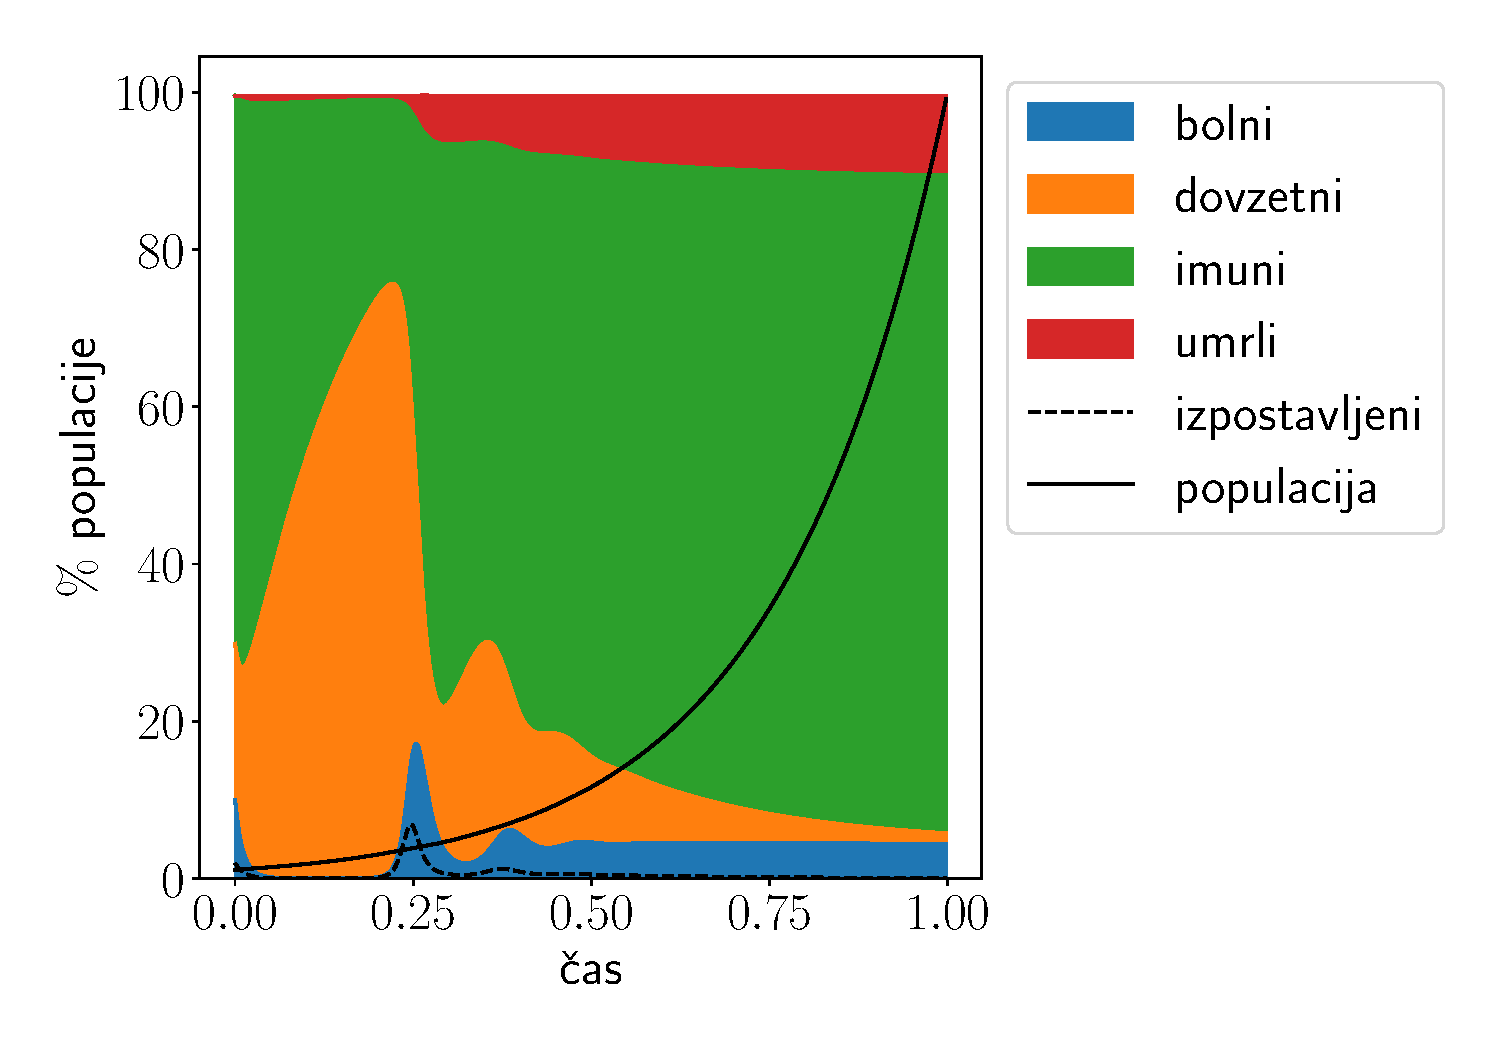
\includegraphics[width=\textwidth]{4.nal slike/smrti_rojstva_zanimivo.pdf}
        \caption{Zanimiv primer za $R_0=1$, $I_0=0,01$, $M_0=0,1$, $N_0=0,05$. Vrh  17,1 \% $\tau = 0,254$, obolelih 38}
        \label{fig:lep_primer}
    \end{subfigure}
    \begin{subfigure}[b]{0.5\textwidth}
        \centering
        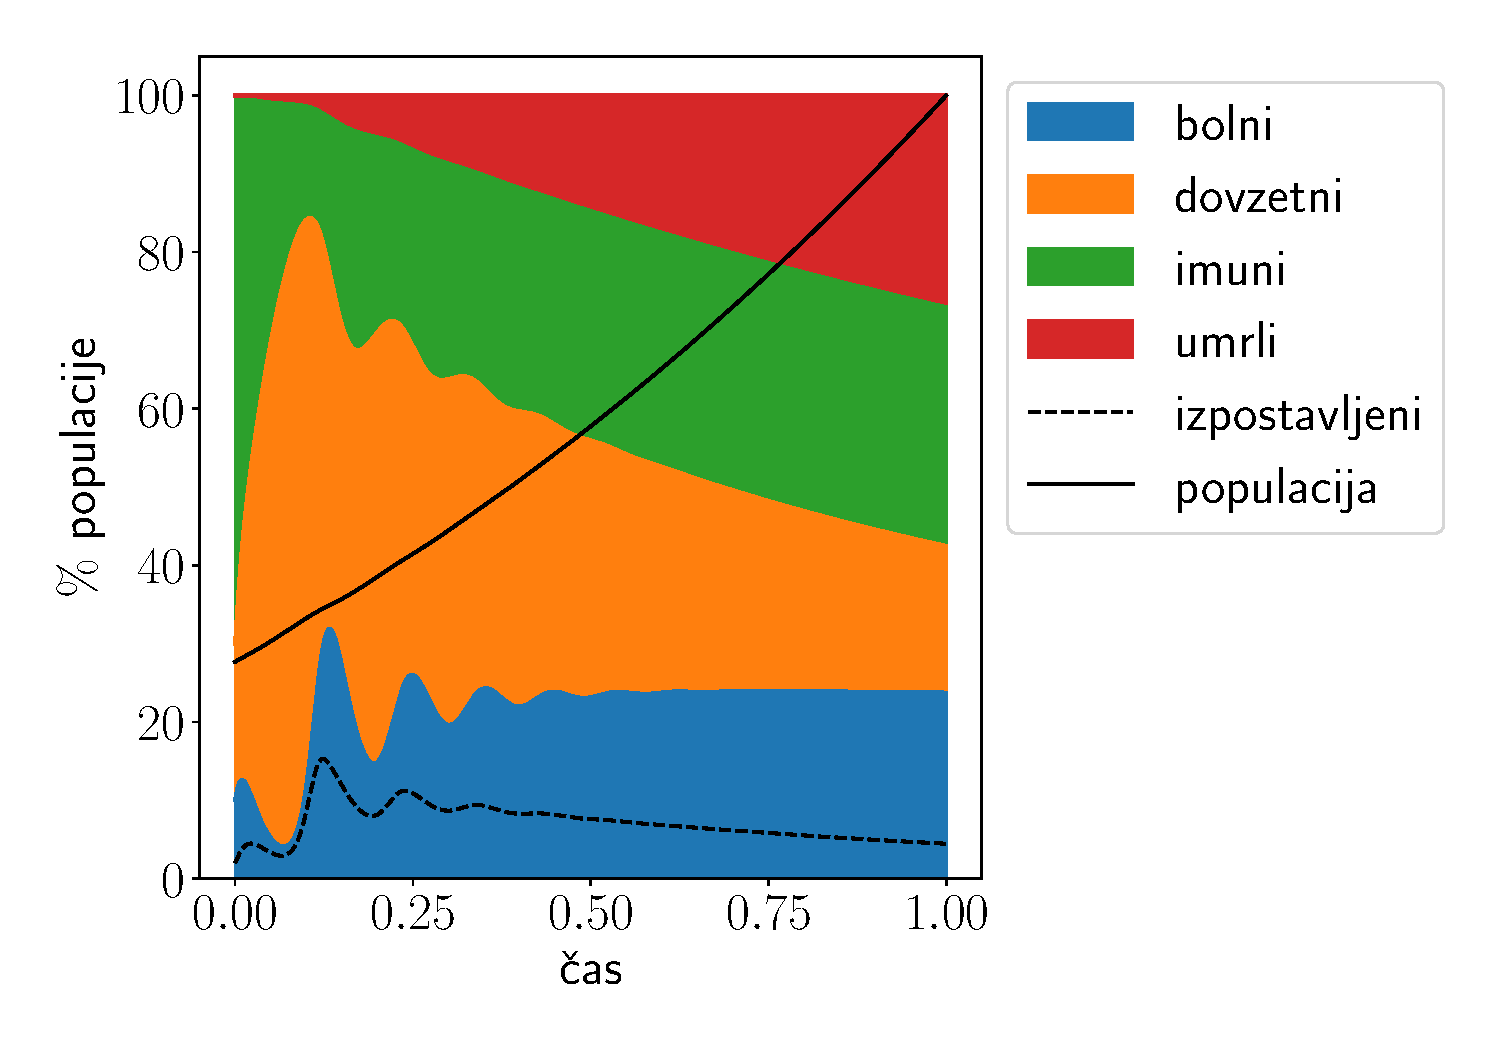
\includegraphics[width=\linewidth]{4.nal slike/stadiji.pdf}
        \caption{Uporaba treh stadijev okužbe. Vrh 31
        ,9 \% $\tau = 0,133$, 1082 obolelih. $\alpha = 1,5$, $\beta_1 = 1$, $\beta_2=0,2$,$\beta_3=0,8$,$\gamma=0,1$,$\delta=\varepsilon=0,01$}
        \label{fig:stadiji}
    \end{subfigure}
\end{centering}
\caption{Možnost modeliranja ciklične epidemije}
\end{figure}
Na spodnjih slikah je opazno, da bolj kompleksi modeli dajo zanimivejše rezultate. Črta z oznako izpostavljeni predstavlja delež dovzetne populacije, ki je v stiku z okuženo. Iz poteka izpostavljenosti je že moč sklepati o časovni lokaciji vrha epidemije in jakosti okužb. Debela črna črta z nazivom populacija pa predstavlja spremembo velikosti populacije zaradi rojstev. Na slikah \ref{fig:smrti} \ref{fig:smrti_rojstva} je opazno, da delež mrtvih ves čas narašča, od vrha epidemije na sliki \ref{fig:smrti} delež bolnih pada proti nič, medtem ko se pri primeru \ref{fig:smrti_rojstva} število bolnih ustali na neničelni vrednosti. Na model opisan z enačbo \ref{eqn:1} vplivamo le z parametrom $\alpha$, ki določa hitrost naraščanja bolnih, na \ref{eqn:3} pa lahko vplivamo le z $R_0$, ki učinkuje enako, vendar v tem primeru vpliva tudi na stabilno lego, torej delež bolnih pri $t \to \infty$. Pri enačbi \ref{eqn:2} lahko že bolje popišemo epidemijo, saj nam parametra $R_0$ in $I_0$ omogočata modelirati vrh. Implementacija rojstev in smrti lahko že tvori kompleksnejše simulacije, lep primer je slika \ref{fig:lep_primer}, kjer smo s parametri uspeli zamakniti vrh epidemije in dobiti celo več vrhov.

Na spodnjih slikah je očitno, da je ključen parameter epidemije reprodukcijsko število. Ta predvsem vpliva na obliko vrha. Na slikah \ref{fig:reprodukcijsko_št} in \ref{fig:odvisnost_čas_vrh} je to še posebej opazno, saj pri nizkih $R_0$ vrh predstavljajo začetni pogoji, pravi vrh se razvije šele pri nekem mejnem $R_0$, ki je odvisen tudi od ostalih parametrov. Zanimivo je, da se čas vrha pri večanju $R_0$ krajša. Hkrati pa je iz ostalih slik razvidno, da se takrat povečuje tudi število obolelih in velikost vrha. Precepljenost, upoštevana v začetnih pogojih pričakovano vpliva na nižanje vrha in obolelih. Parameter $I_0$ vpliva le na prehod imunih v dovzetne. Zanimivo je, da se število obolelih za velike $R_0$ in $I_0$ ustali.
\begin{figure}[ht!]
\begin{centering}
    \begin{subfigure}[b]{0.5\textwidth}
        \centering
        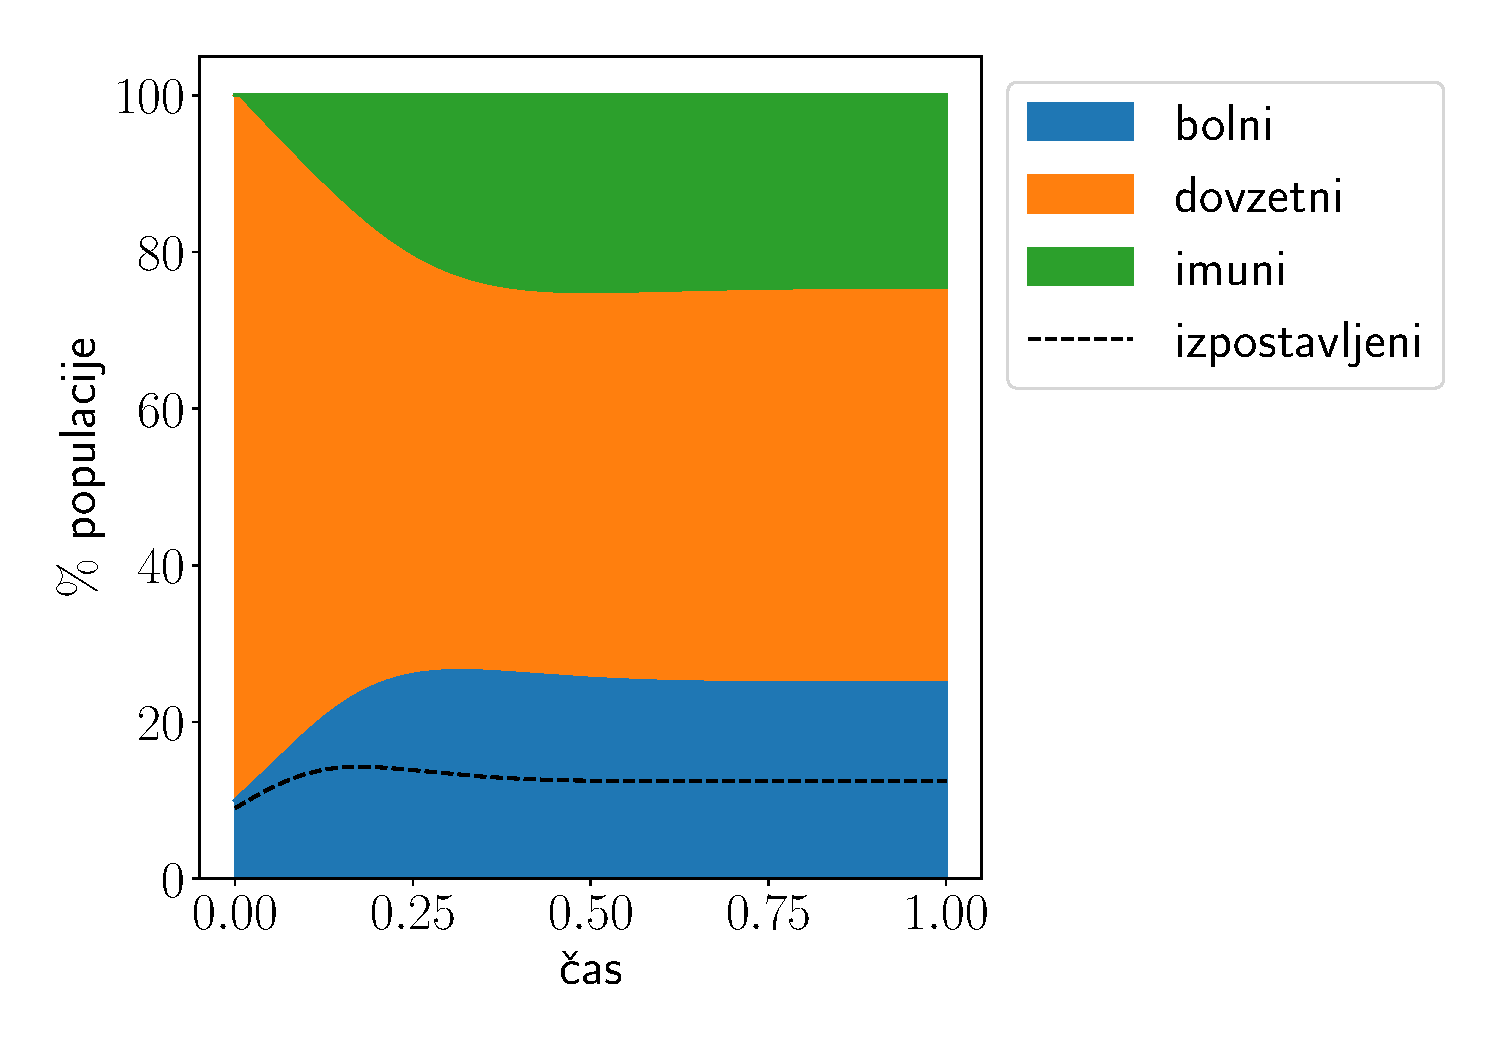
\includegraphics[width=\linewidth]{4.nal slike/ozdravitev_R2_I1.pdf}
        \caption{$R_0=2$, vrh pri 26,5 \% in $\tau = 0,316$, obolelih je 239}
    \end{subfigure}
    \begin{subfigure}[b]{0.5\textwidth}
        \centering
        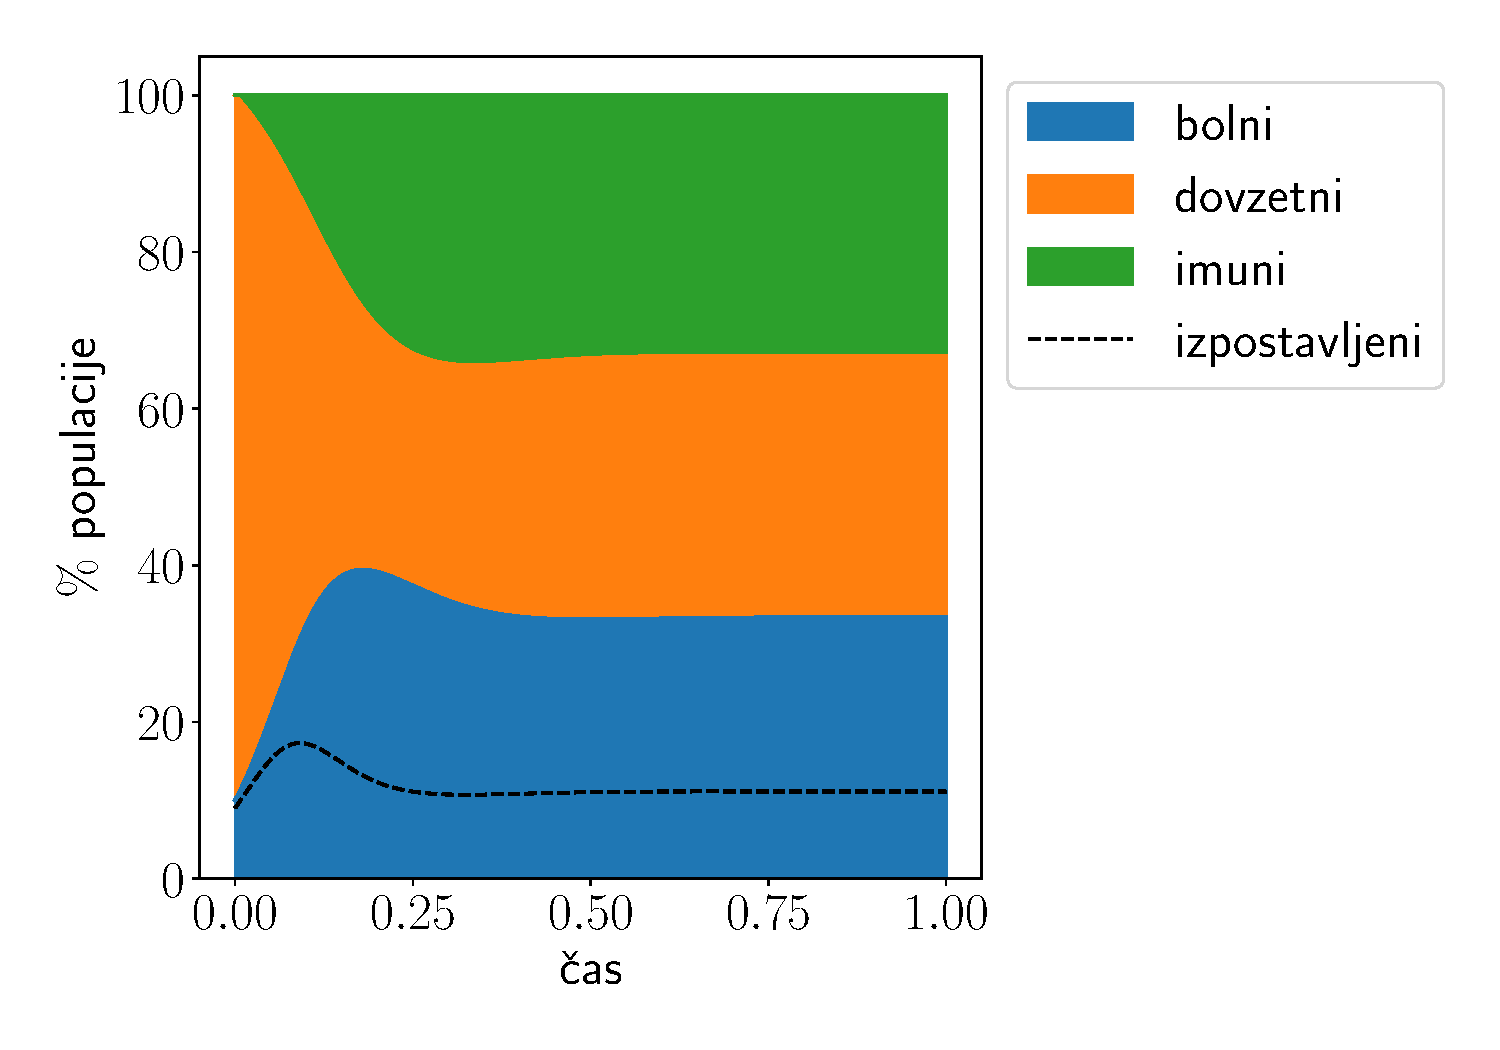
\includegraphics[width=\linewidth]{4.nal slike/ozdravitev_R3_I1.pdf}
        \caption{$R_0=3$, vrh pri 39,4 \% in $\tau = 0,180$, obolelih je 329}
    \end{subfigure}
    \begin{subfigure}[b]{0.5\textwidth}
        \centering
        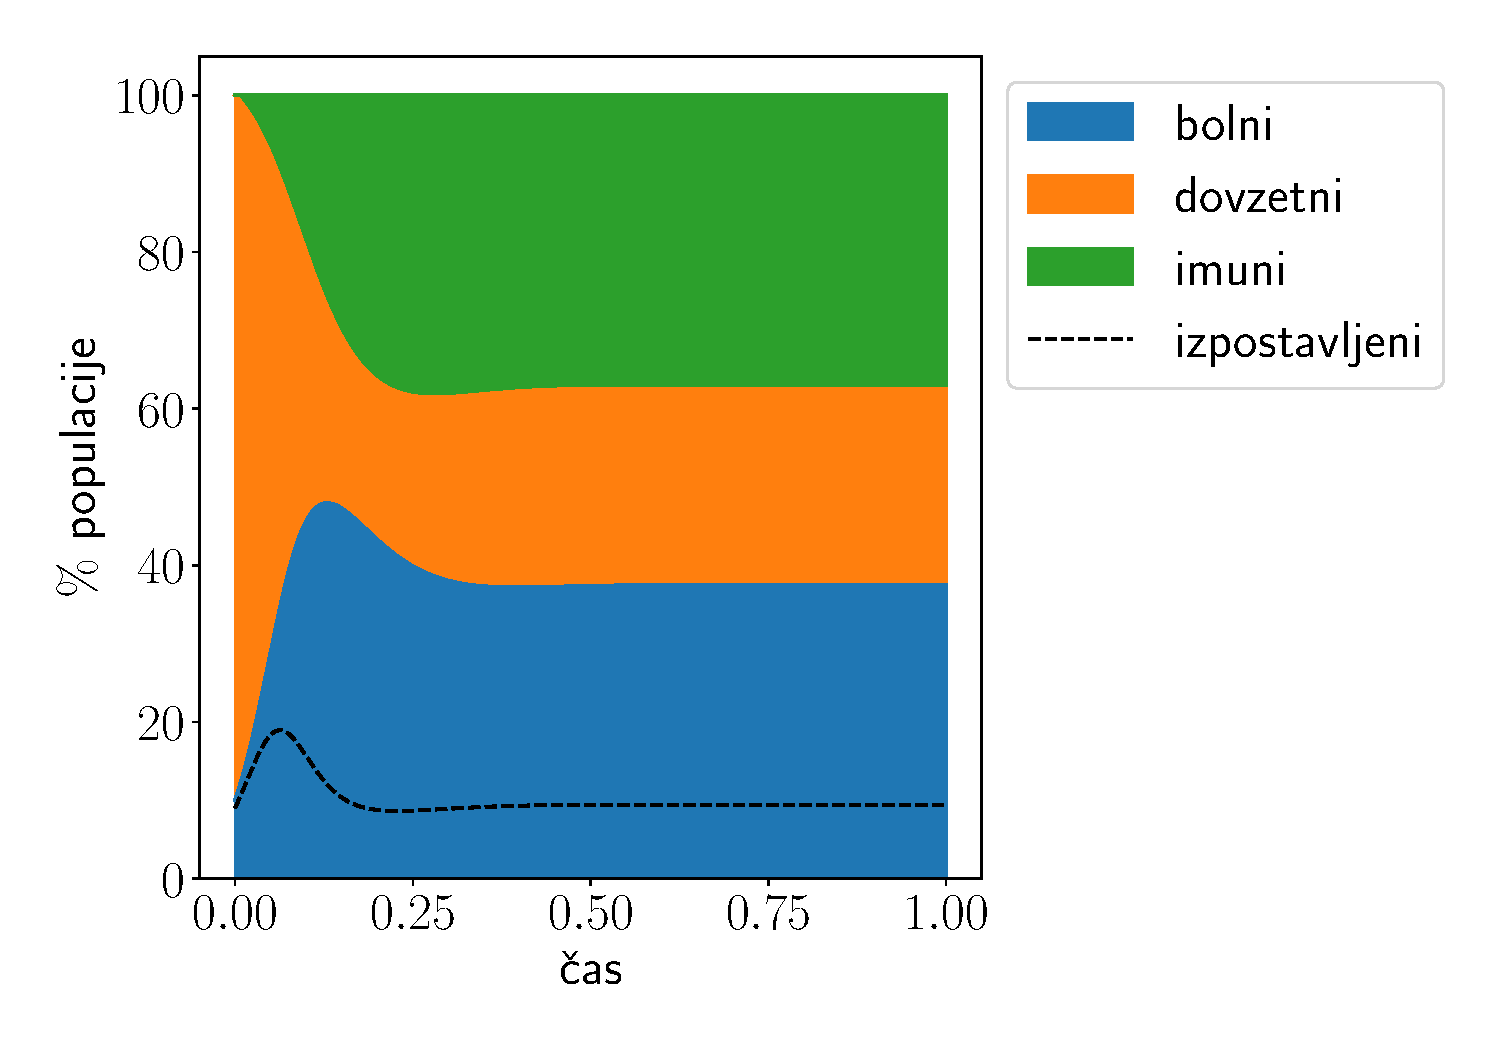
\includegraphics[width=\linewidth]{4.nal slike/ozdravitev_R4_I1.pdf}
        \caption{$R_0=4$, vrh pri 47,9 \% in $\tau = 0,130$, obolelih je 377}
    \end{subfigure}
    \begin{subfigure}[b]{0.5\textwidth}
        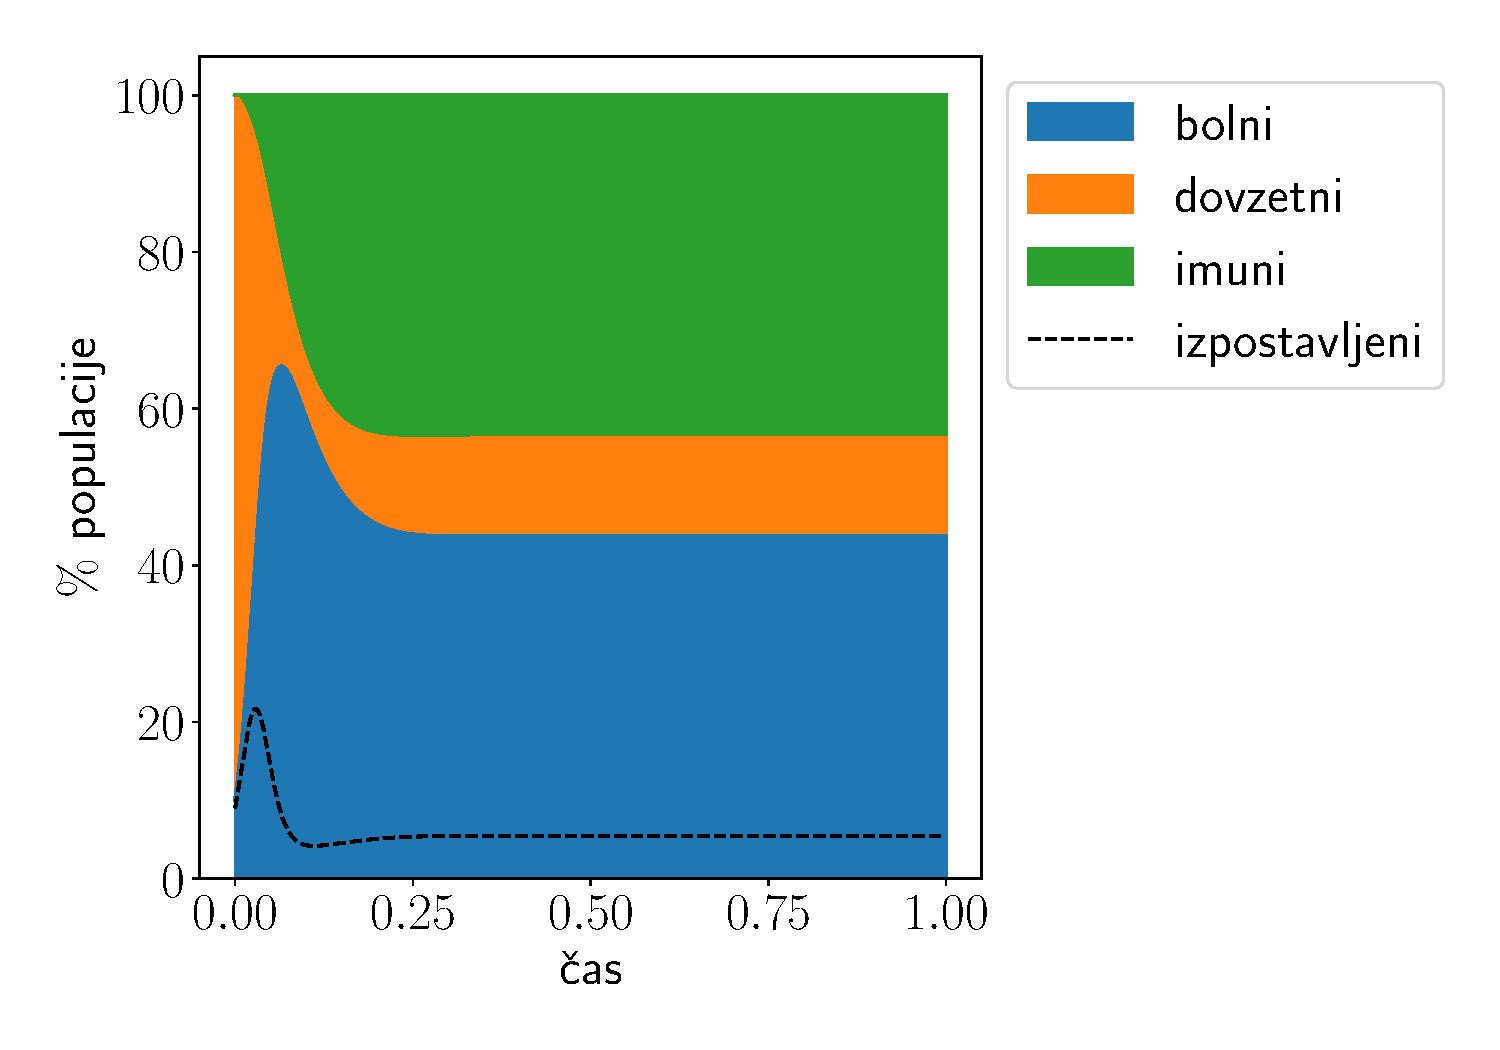
\includegraphics[width=\linewidth]{4.nal slike/ozdravitev_R8_I1.pdf}
        \caption{$R_0=8$, vrh pri 65,4 \% in $\tau = 0,065$, obolelih je 449}
    \end{subfigure}
\end{centering}
\caption{Simulacije po enačbi \ref{eqn:4}}
\label{fig:reprodukcijsko_št}
\end{figure}
\begin{figure}[ht!]
\begin{centering}
    \begin{subfigure}[b]{0.5\textwidth}
        \centering
        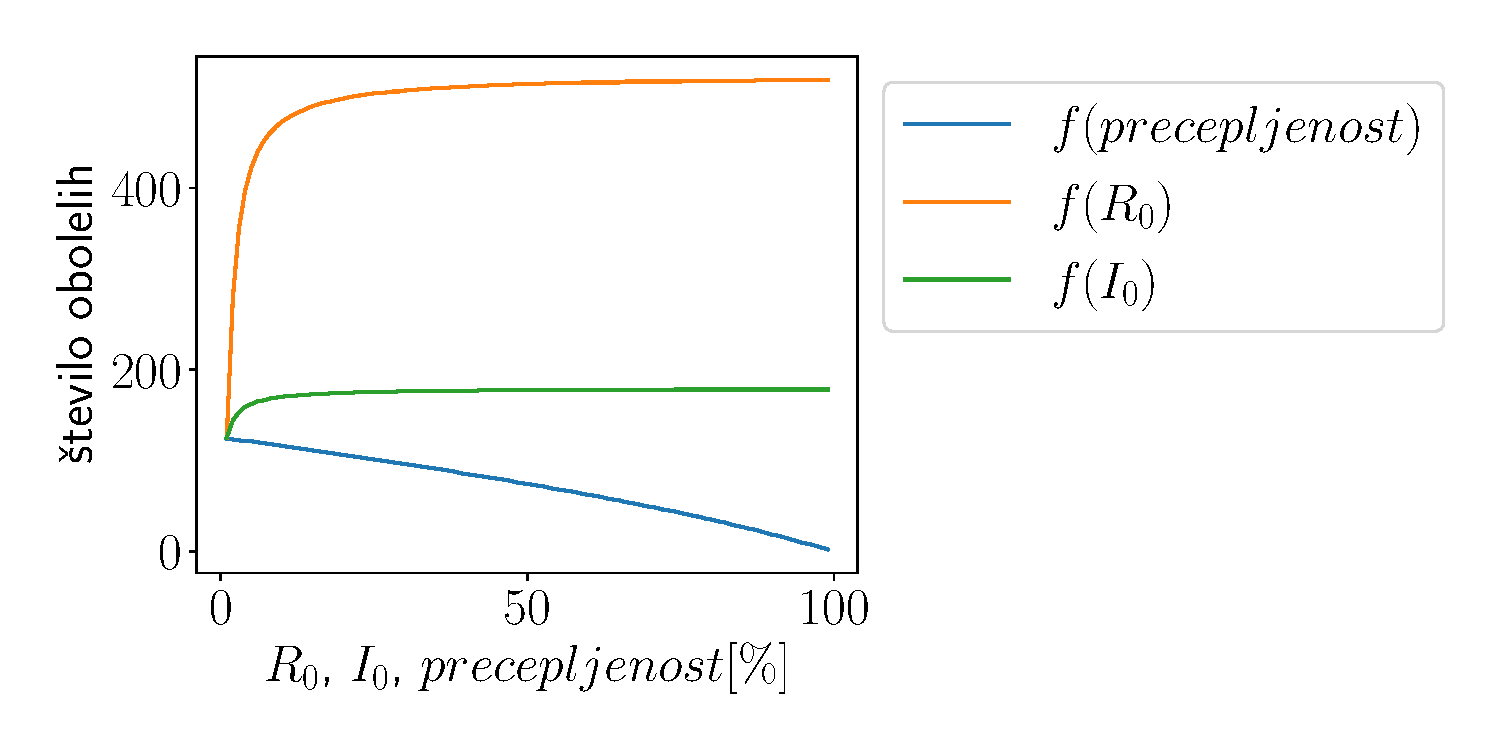
\includegraphics[width=\linewidth]{4.nal slike/št_obolelih_odvisnost.pdf}
        \caption{Odvisnost števila obolelih od $R_0$, $I_0$ in precepljenosti}
        \label{fig:odvisnost_oboleli}
    \end{subfigure}
    \begin{subfigure}[b]{0.5\textwidth}
        \centering
        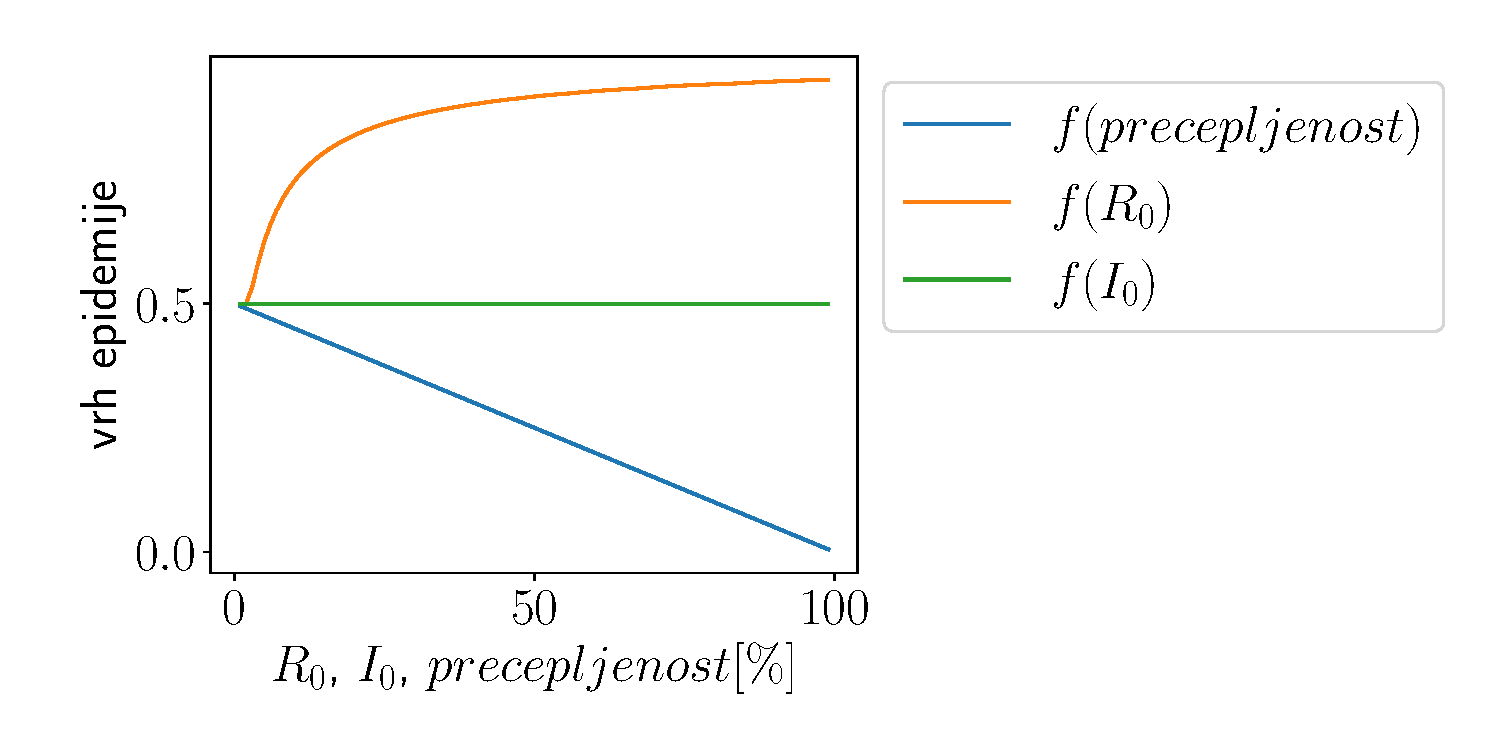
\includegraphics[width=\linewidth]{4.nal slike/vrh_odvisnost.pdf}
        \caption{Odvisnost vrha epidemije od $R_0$, $I_0$ in precepljenosti}
        \label{fig:odvisnost_vrh}
    \end{subfigure}
    \begin{subfigure}[b]{0.4\textwidth}
        \centering
        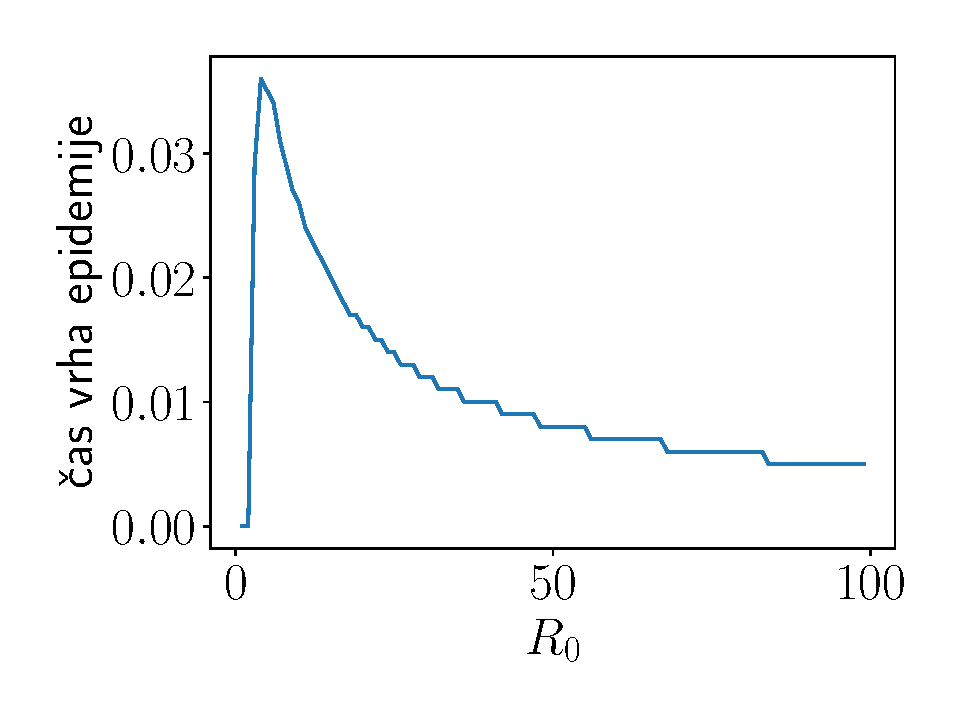
\includegraphics[width=\linewidth]{4.nal slike/čas_vrh_odvisnost.pdf}
        \caption{Odvisnost časa nastopa vrha epidemije od $R_0$. Od $I_0$ in precepljenosti je neodvisen.}
        \label{fig:odvisnost_čas_vrh}
    \end{subfigure}
\end{centering}
\caption{Vplivi na parametre epidemija. Uporabljen je model z imuno ozdravitvijo z enačbo \ref{eqn:4}}
\end{figure}

\newpage
\vfill
x
\newpage

\section{Model zajci-lisice}

Model Lotka-Volterra se v brezdimenzijski obliki glasi:
\begin{align}
    \dot z &= p \, z \, (1-l) \\ \nonumber
    \dot l &= \frac{l}{p} \, (z-1)
\end{align}
kjer je $p$ edini prosti parameter. Zastojni točki se nahajata na $(0,0)$ in $(1,1)$.

\begin{figure}[ht!]
\begin{centering}
    \begin{subfigure}{0.5\textwidth}
        \centering
        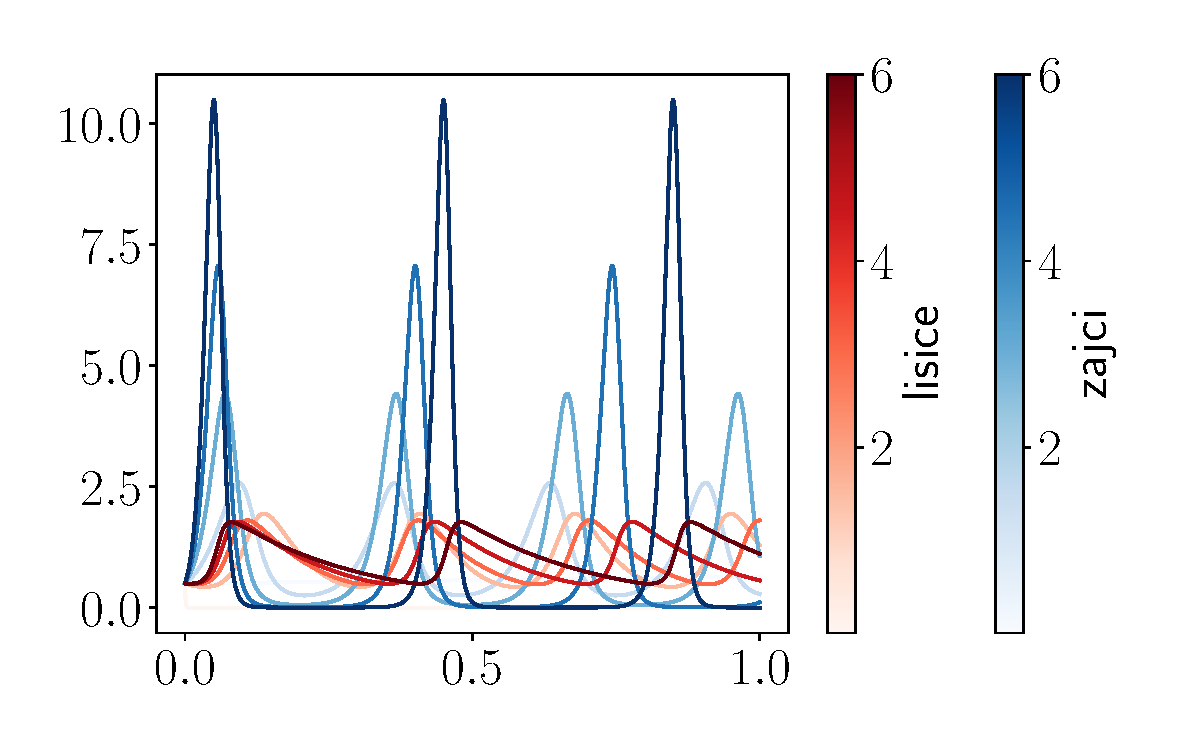
\includegraphics[width=\linewidth]{4.nal slike/zajci_lisice.pdf}
        \caption{Odvisnost populacije zajcev in lisic od $p$}
        \label{fig:odv_p}
    \end{subfigure}
    \begin{subfigure}{0.5\textwidth}
        \centering
        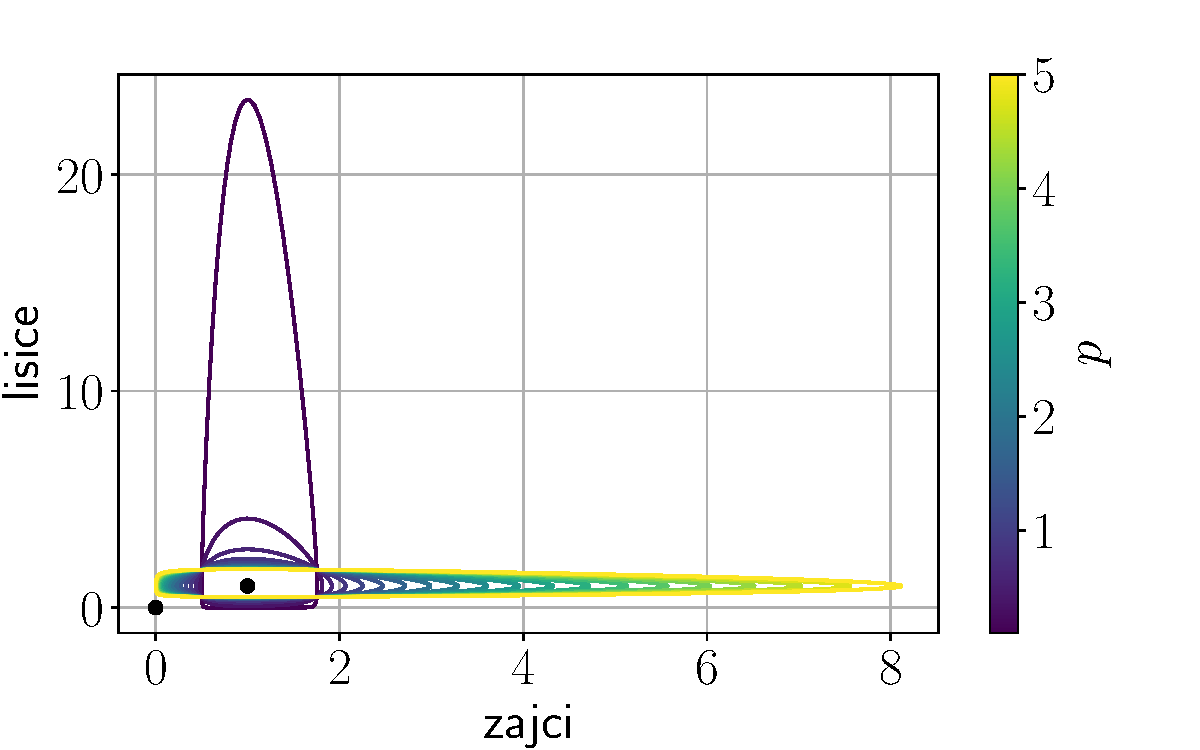
\includegraphics[width=\linewidth]{4.nal slike/zajci_lisice_fazni.pdf}
        \caption{Fazni diagram v odvisnosti od $p$ okoli zastojne točke}
        \label{fig:odv_p}
    \end{subfigure}
\end{centering}
\caption{Standardni model zajci-lisice}
\end{figure}
\begin{figure}[ht!]
\begin{centering}
    \begin{subfigure}{0.5\textwidth}
        \centering
        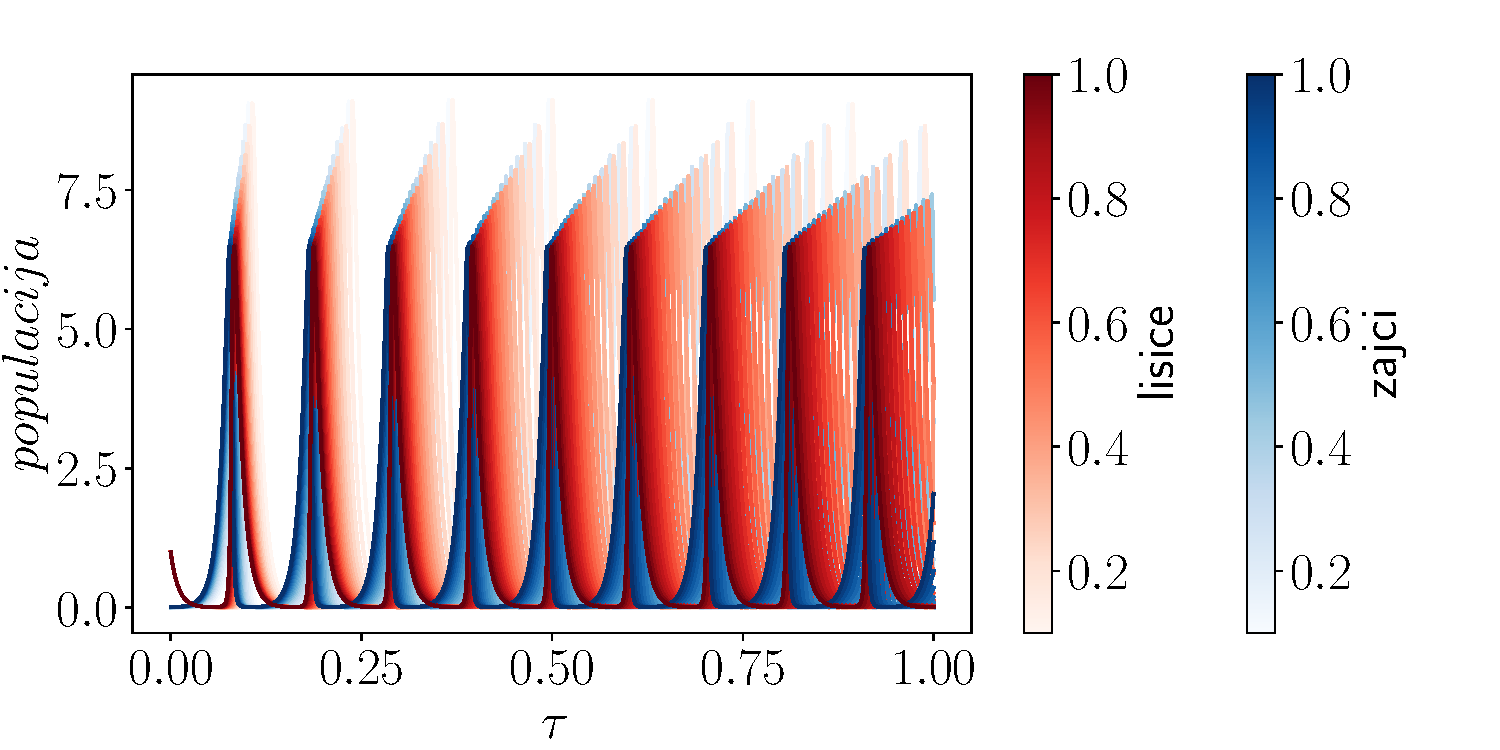
\includegraphics[width=\linewidth]{4.nal slike/zajci_malo.pdf}
    \end{subfigure}
    \begin{subfigure}{0.5\textwidth}
        \centering
        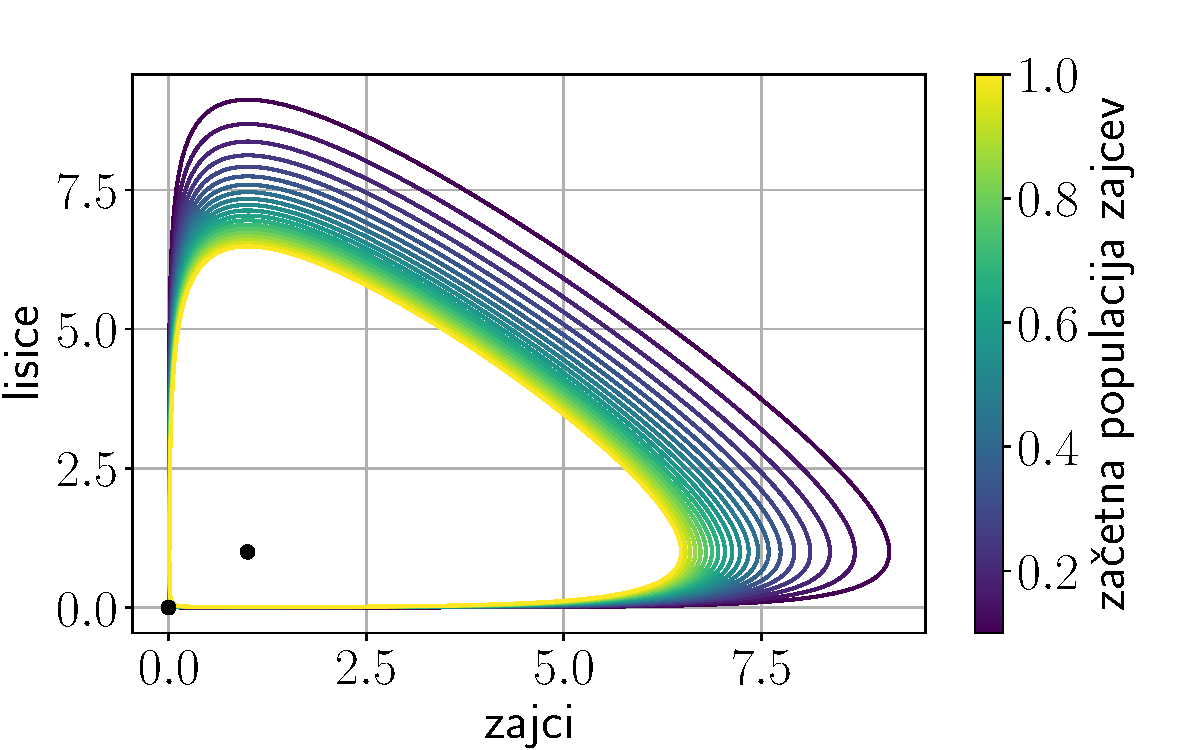
\includegraphics[width=\linewidth]{4.nal slike/zajci_malo_fazni.pdf}
    \end{subfigure}
\end{centering}
\caption{Primer z malo populacijo zajcev}
\end{figure}
\begin{figure}[ht!]
\begin{centering}
    \begin{subfigure}{0.5\textwidth}
        \centering
        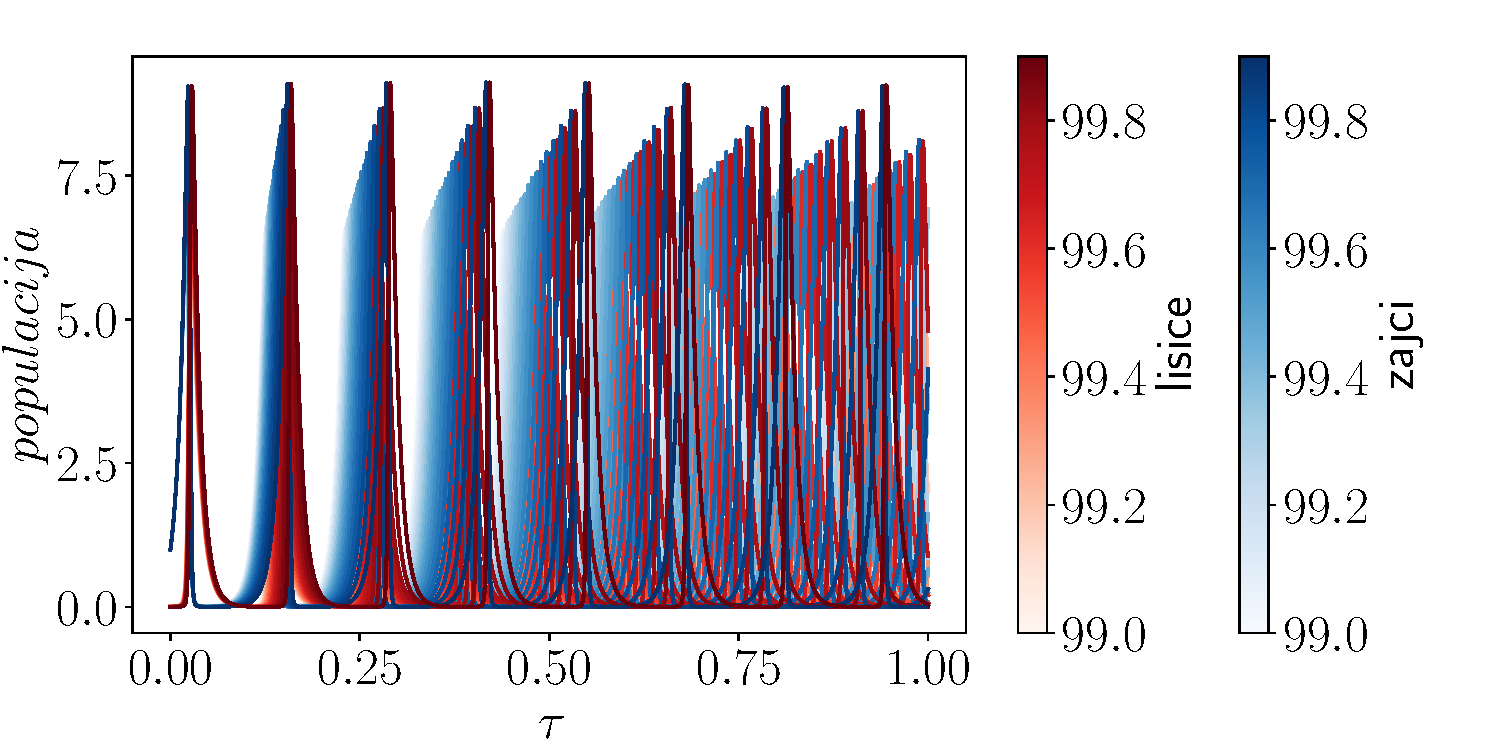
\includegraphics[width=\linewidth]{4.nal slike/zajci_veliko.pdf}
    \end{subfigure}
    \begin{subfigure}{0.5\textwidth}
        \centering
        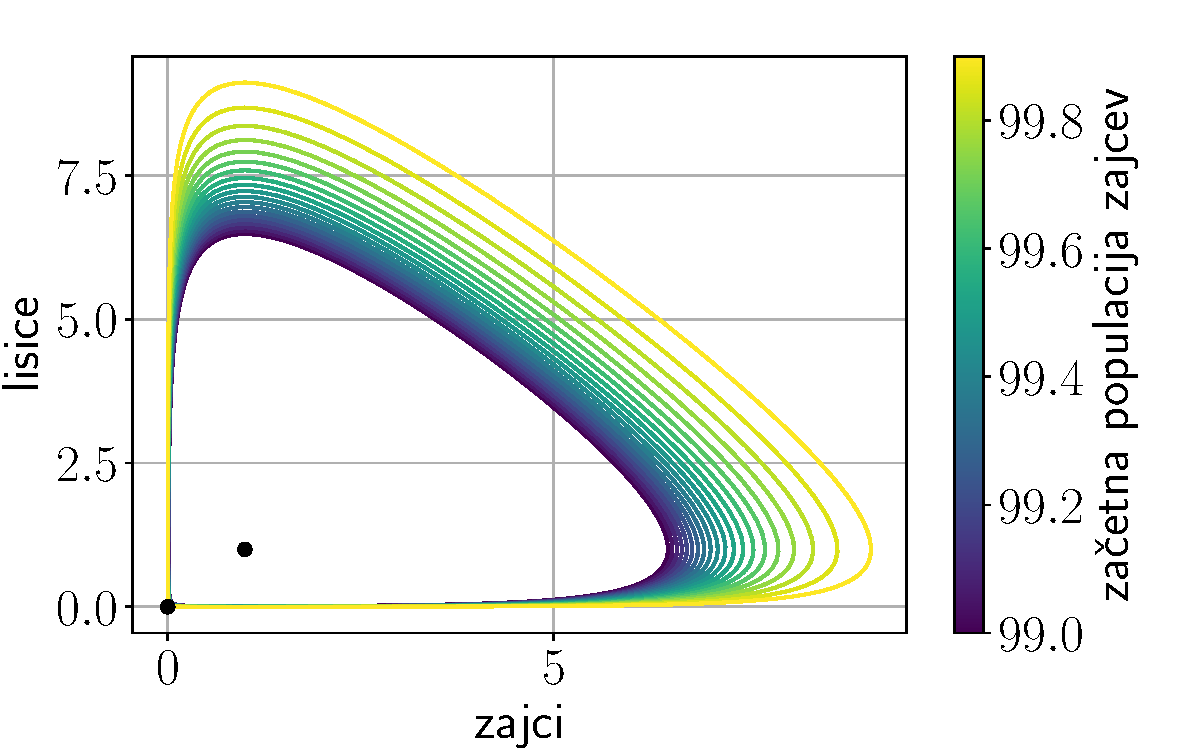
\includegraphics[width=\linewidth]{4.nal slike/zajci_veliko_fazni.pdf}
    \end{subfigure}
\end{centering}
\caption{Primer z veliko populacijo zajcev}
\end{figure}

\newpage
\section{Model laserja}

V primeru analize laserja rešujemo sistem dveh NDE v brezdimenzijski obliki:
\begin{align}
    \dot A &= r - p \, A \, (F+1) \\ \nonumber
    \dot F &= \frac{F}{p} \, (A-1)
\end{align}
kjer $r$ predstavlja črpanje, $p$ pa parameter lastnosti laserja. Tako dobimo tudi zastojni točki $\left( \frac{r}{p}, 0 \right)$ in $\left( 1, \frac{r}{p} - 1 \right)$.

Slika \ref{fig:laser} prikazuje delovanje laserja. Opazimo, da pri visokem parametru $p$ laser ugasne ob premajhnem črpanju $r$, ki vpliva predvsem na stabilno lego populacij atomov in fotonov. Pri nizkem $p$ prihaja do pojava oscilacij fotonov. Na sliki \ref{fig:r_0.4} vidimo, da pri napačnih parametrih laserja pride do pojava oscilacij, ki sicer vodijo do konstantnega delovanja laserja pri večji populaciji fotonov za nižje $p$.

Zastojne točke so najbolje vidne na sliki \ref{fig:laser}, kjer zaradi nazornosti prikaza točke na abscisi niso prikazane.
\begin{figure}[ht!]
\begin{centering}
    \begin{subfigure}{0.5\textwidth}
        \centering
        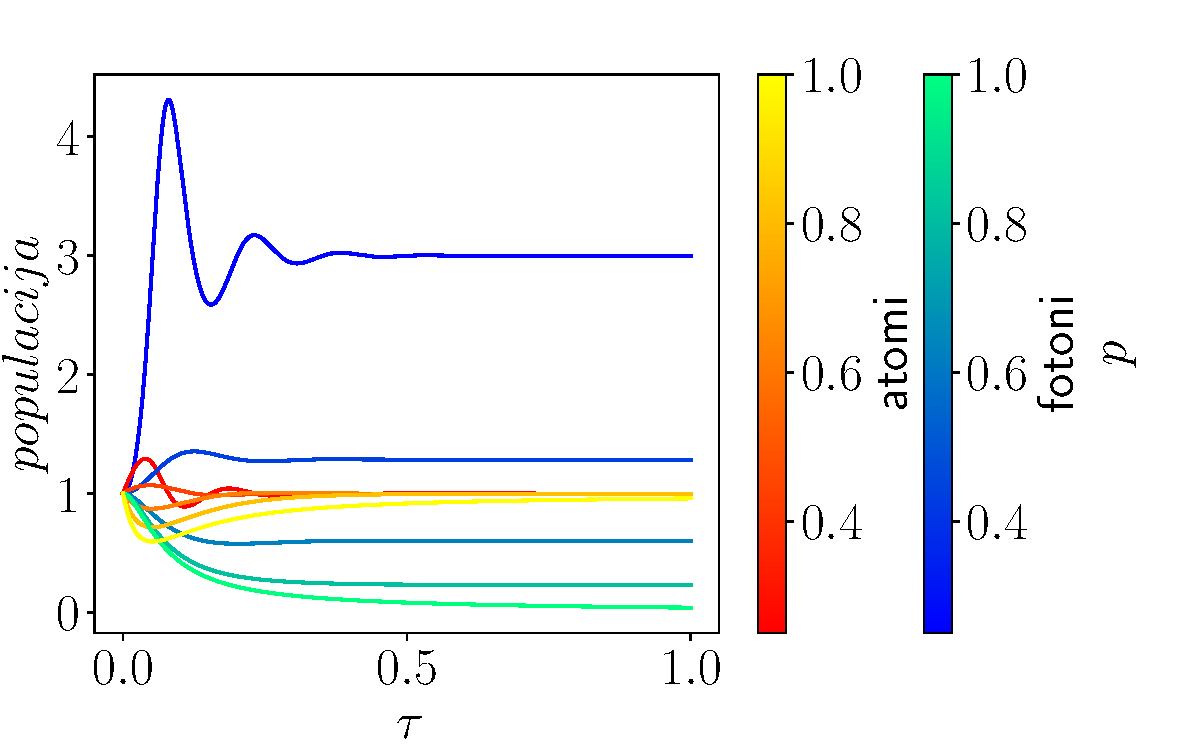
\includegraphics[width=\linewidth]{4.nal slike/fotoni_atomi.pdf}
        \caption{Gibanje populacije fotonov in atomov v odvisnosti od $p$ pri $r=1$}
        \label{fig:fotoni_atomi}
    \end{subfigure}
    \begin{subfigure}{0.5\textwidth}
        \centering
        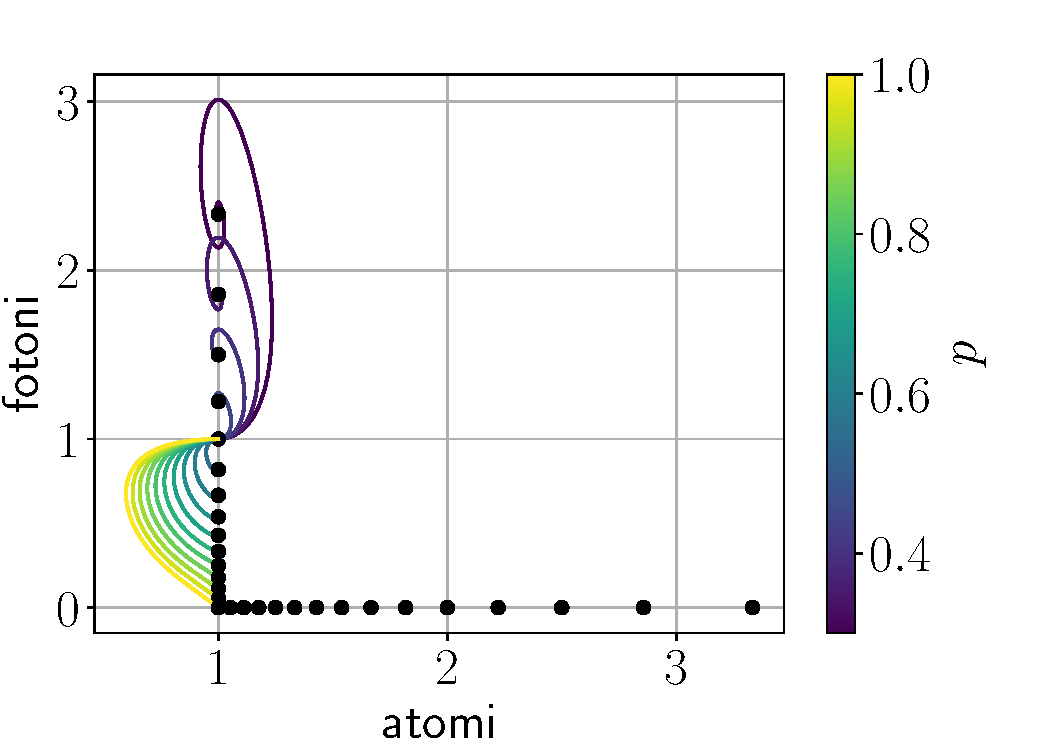
\includegraphics[width=\linewidth]{4.nal slike/fotoni_atomi_fazni_visoki_p.pdf}
        \caption{Fazni diagram v odvisnosti od $r$ pri $p=1$}
        \label{fig:fotoni_atomi}
    \end{subfigure}
    \begin{subfigure}{0.5\textwidth}
        \centering
        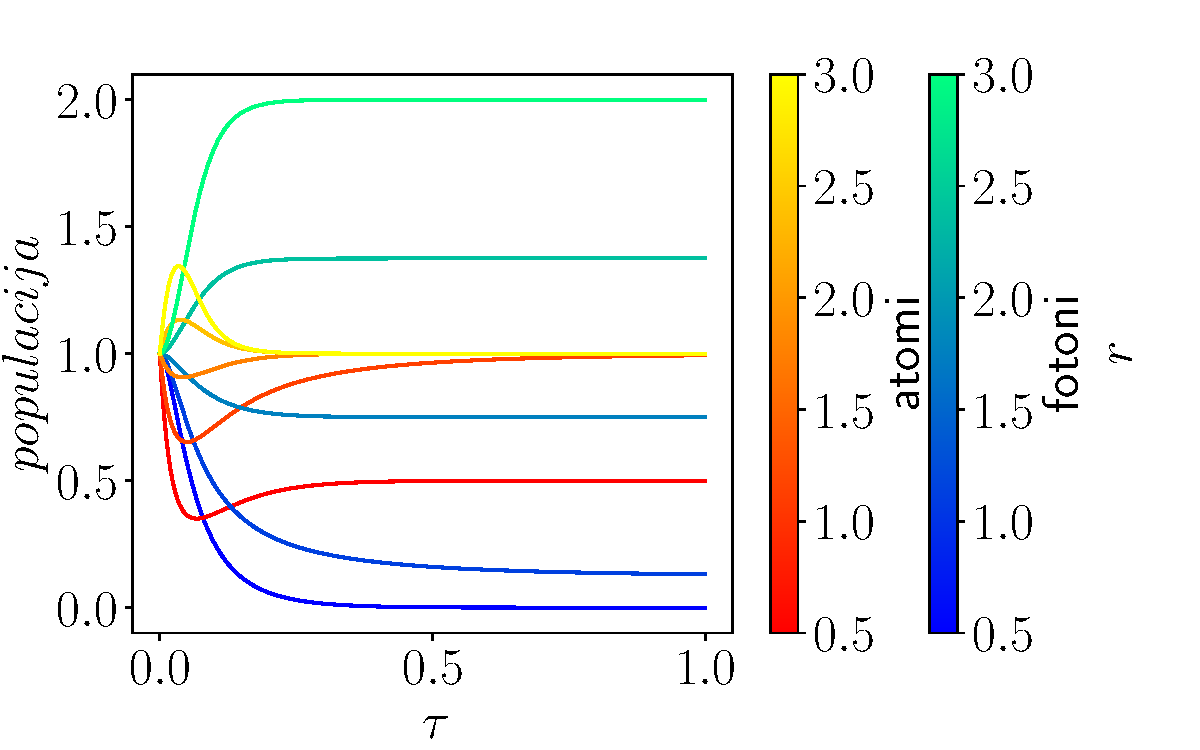
\includegraphics[width=\linewidth]{4.nal slike/fotoni_atomi_r.pdf}
        \caption{Gibanje populacije fotonov in atomov v odvisnosti od $r$ pri $p=1$}
        \label{fig:fotoni_atomi}
    \end{subfigure}
    \begin{subfigure}{0.5\textwidth}
        \centering
        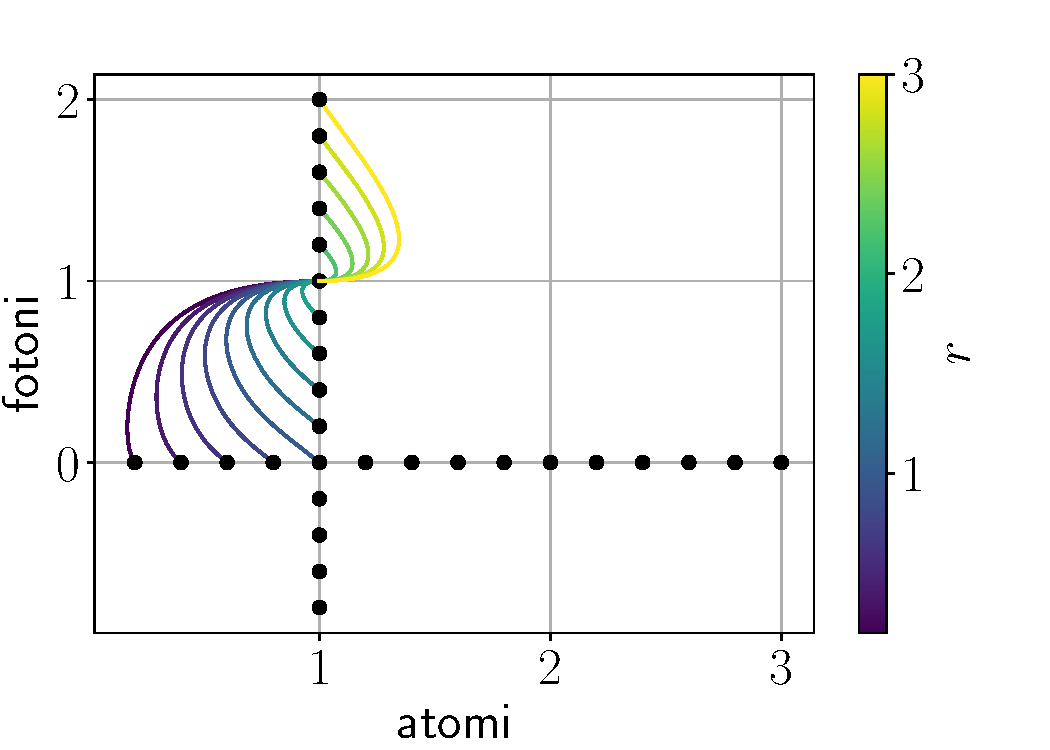
\includegraphics[width=\linewidth]{4.nal slike/fotoni_atomi_fazni_r.pdf}
        \caption{Fazni diagram v odvisnosti od $r$ pri $p=1$}
        \label{fig:fotoni_atomi}
    \end{subfigure}
    \begin{subfigure}{0.5\textwidth}
        \centering
        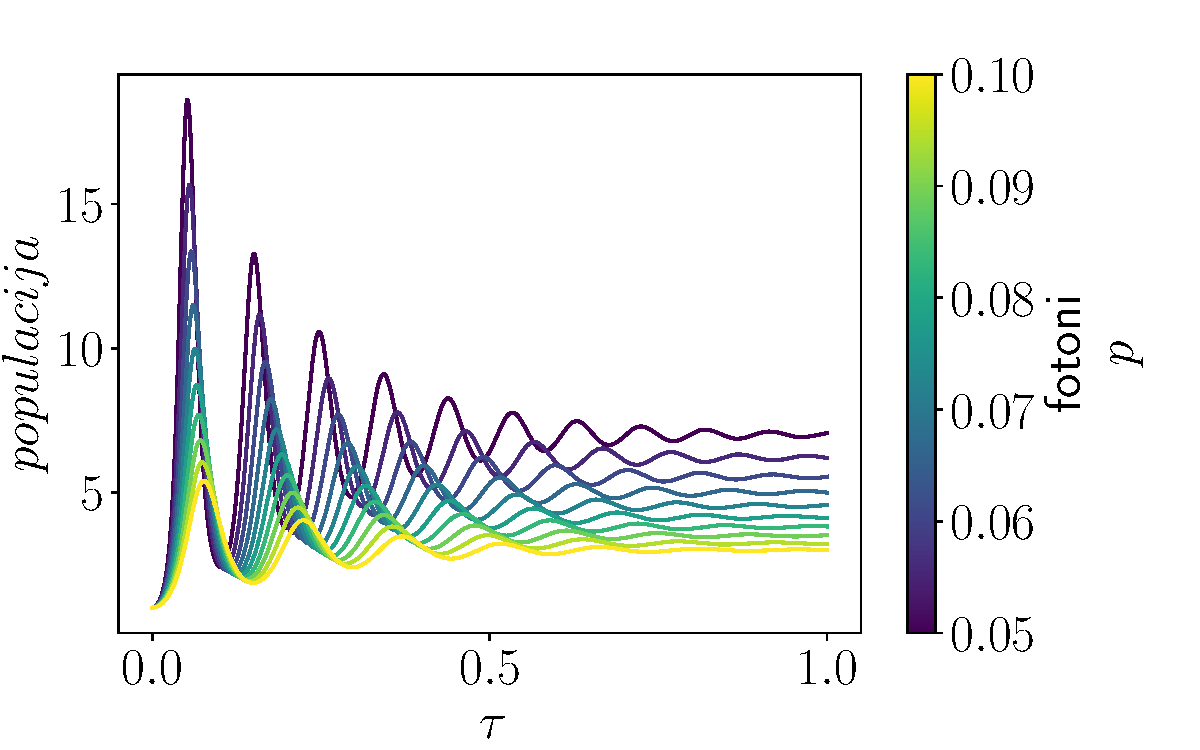
\includegraphics[width=\linewidth]{4.nal slike/fotoni_atomi_r0.4.pdf}
        \caption{Oscilacije populacije fotonov pri $r=0,4$ za $0,05<p<0,1$}
        \label{fig:r_0.4}
    \end{subfigure}
    \begin{subfigure}{0.5\textwidth}
        \centering
        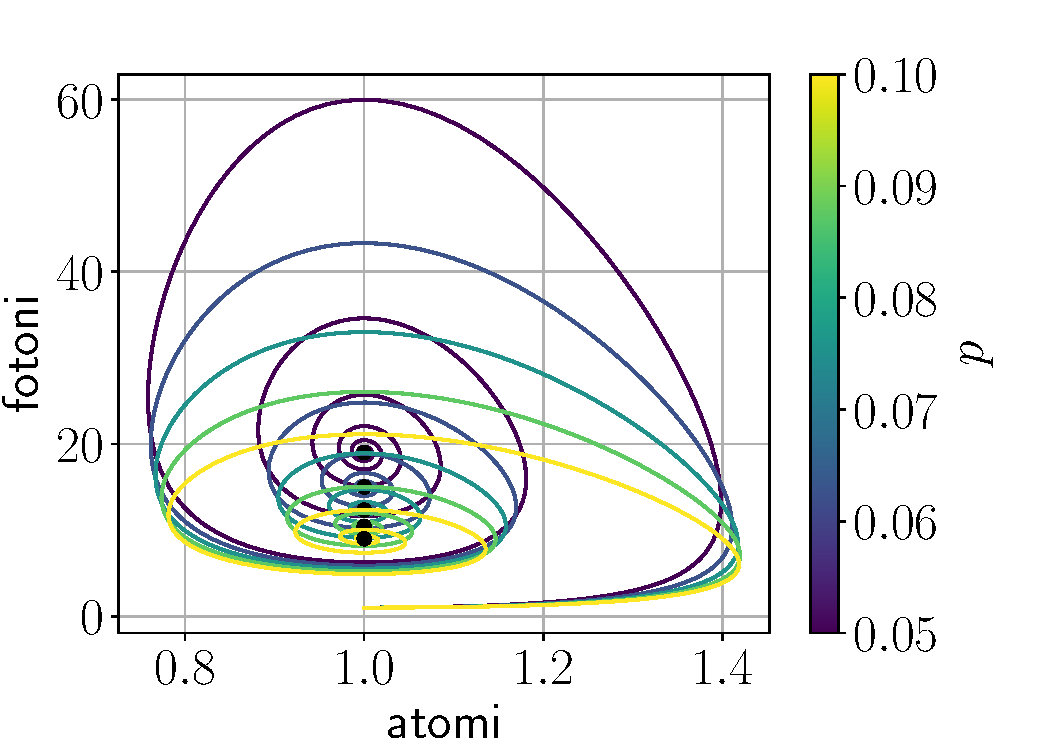
\includegraphics[width=\linewidth]{4.nal slike/fotoni_atomi_fazni_nizki_p.pdf}
        \caption{Fazni diagram pri $r=0,4$ za $0,05<p<0,1$}
    \end{subfigure}
\end{centering}
\caption{Delovanje laserja}
\label{fig:laser}
\end{figure}

Na sliki \ref{fig:ampl_frek} vidimo, da frekvenca in amplituda oscilacij narašča z manjšanjem $p$, kar je razvidno tudi iz slike \ref{fig:laser}. Vrh pri $p=0,5$ je verjetno numerična napaka, saj sem frekvence določeval s pomočjo brze Fouriereve transformacije FFT.
\begin{figure}[ht!]
    \centering
    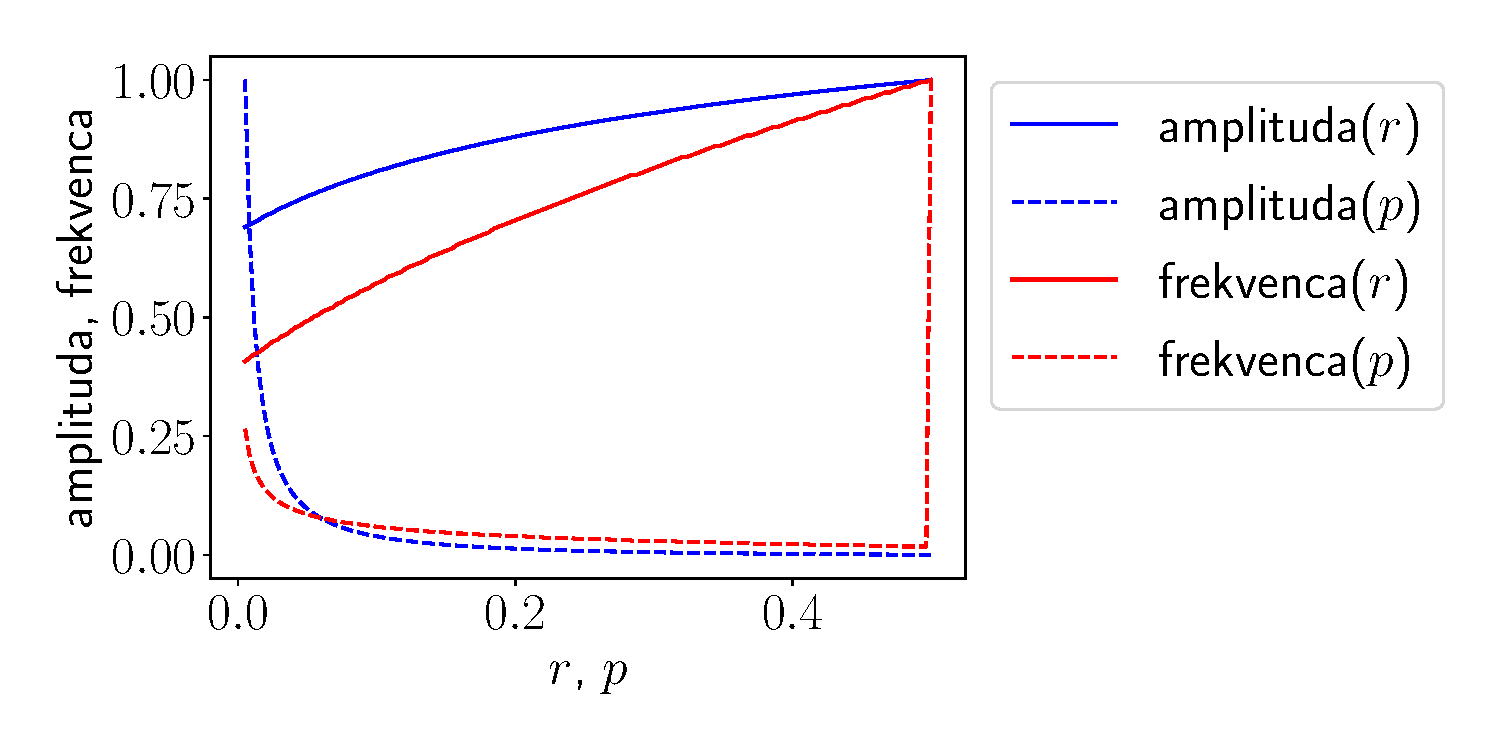
\includegraphics[width=0.7\textwidth]{4.nal slike/amplituda_frek.pdf}
    \caption{Odvisnost amplitude in frekvence laserskih oscilacij od $p$ in $r$}
    \label{fig:ampl_frek}
\end{figure}